% PLEASE FILL IN THE PLACEHOLDERS <...>
%
% Bachelorarbeit von Henry He
% Bachelor thesis of Henry He
%
% Title: AoI-based Scheduling for Networked Control Systems over Gilbert-Elliot Channel
%        
%
\documentclass[12pt,a4paper]{report}

%%%%%%%%%%%%%%%%%%%%%%%%%%%%%%%%%%%%%%%%%%%%%%%%%%%%%%%%%%%%

% PACKAGES:

% Define typearea
% a) Use automatic:
\usepackage[BCOR1cm]{typearea}
% b) Or use fixed: 
%\usepackage{geometry}
%\geometry{left=1.5cm,textwidth=18.5cm,top=1.5cm,textheight=26.5cm}

% Use German :
%\usepackage[ngerman]{babel}
% Use list of tabels, etc. in table of contents:
\usepackage{tocbibind}
% German paragraph skip
\usepackage{parskip}
% Encoder:
\usepackage[utf8]{inputenc}
% Use A4-paper efficiently:
\usepackage{a4wide}
% Index-generation
\usepackage{makeidx}
% Einbinden von URLs:
\usepackage{url}
% Include Graphic-files:
\usepackage{graphicx}
\graphicspath{ {./figures/} }
% Include .eps-files (needed also for the LKN-logo):
\usepackage[outdir=./figures/]{epstopdf}
\epstopdfDeclareGraphicsRule{.pdf}{png}{.png}{convert #1 \OutputFile}
\DeclareGraphicsExtensions{.png,.pdf}
% Special \LaTex symbols (e.g. \BibTeX):
\usepackage{doc}
% Include doc++ generated tex-files:
%\usepackage{docxx}
\usepackage{amsmath,amssymb,amsfonts}
\usepackage{array}
\usepackage{tikz}
\usetikzlibrary{automata, positioning, shapes, arrows}
% Include PDF links
\usepackage[bookmarks=true, hidelinks]{hyperref}

%%%%%%%%%%%%%%%%%%%%%%%%%%%%%%%%%%%%%%%%%%%%%%%%%%%%%%%%%%%%

% OTHER SETTINGS:

% Pagestyle:
\pagestyle{headings}

% Avoid 'overhang':
\sloppy

% Choose language
\newcommand{\setlang}[1]{\selectlanguage{#1}\nonfrenchspacing}

% Import macros:
\definecolor{myred}{RGB}{220,43,25}
\definecolor{mygreen}{RGB}{0,146,64}
\definecolor{myblue}{RGB}{0,143,224}
\definecolor{mygray}{gray}{0.80}
\definecolor{mylightergray}{gray}{0.87}
\definecolor{mylightestgray}{gray}{0.95}



\usepackage{soul}

\newif\ifcomments

\commentstrue
\newcommand{\commentBy}[3]{\textcolor{#1}{\{#2: #3\}}}

\newcommand{\oa}[1]{\textcolor{myred}{#1}}

\newcommand{\mg}[1]{\textcolor{mygreen}{#1}}
\newcommand{\mgrm}[1]{\textcolor{mygreen}{\st{#1}}}
\newcommand{\mgrep}[2]{\textcolor{mygreen}{(#1) can be replaced with: #2}}


% Own Macros
\newtheorem{mydef}{Definition}
\newcommand{\setOfULResources}{\mathcal{R}^{\text{UL}}}
\newcommand{\setOfDLResources}{\mathcal{R}^{\text{DL}}}
\newcommand{\numOfULResources}{\mathsf{R^{\text{UL}}}}
\newcommand{\numOfDLResources}{\mathsf{R^{\text{DL}}}}
\newcommand{\ulResourceConsumption}{r_i^{\text{UL}}}
\newcommand{\dlResourceConsumption}{r_i^{\text{DL}}}
\newcommand{\setOfSamples}{\Xi_i}
\newcommand{\txDelay}{d}
\newcommand{\numLoops}{N}
\newcommand{\bs}{\text{BS}}
\newcommand{\avgAge}{\overline{\Delta}}
\newcommand{\iae}{\Sigma_{e}}
\newcommand{\samplingPeriod}{T^s_i}
\newcommand{\E}{\mathbb{E}}
\newcommand{\tr}{\mathsf{tr}}
\newcommand{\ki}{k_i}
\newcommand{\plant}{\mathcal{P}_i}
\newcommand{\sensor}{\mathcal{S}_i}
\newcommand{\controller}{\mathcal{C}_i}
\newcommand{\estimator}{\mathcal{E}_i}
\newcommand{\errornorm}{\E\left[\left\Vert e_i[k] \right\Vert^2 \right]}
\newcommand{\statespace}{\bm{\mathcal{\bm{S}}}}
\newcommand{\approxstatespace}{\bm{\mathcal{S}}_M}
\newcommand{\minus}{\scalebox{0.75}[1.0]{$\,-\,$}}
\newcommand{\floor}[1]{\left\lfloor #1 \right\rfloor}
\newcommand{\ceil}[1]{\left\lceil #1 \right\rceil}

%%%%%%%%%%%%%%%%%%%%%%%%%%%%%%%%%%%%%%%%%%%%%%%%%%%%%%%%%%%%

\begin{document}

% TITLE:
\thispagestyle{empty}
\newpage

\vspace{5cm}
  \begin{center}
        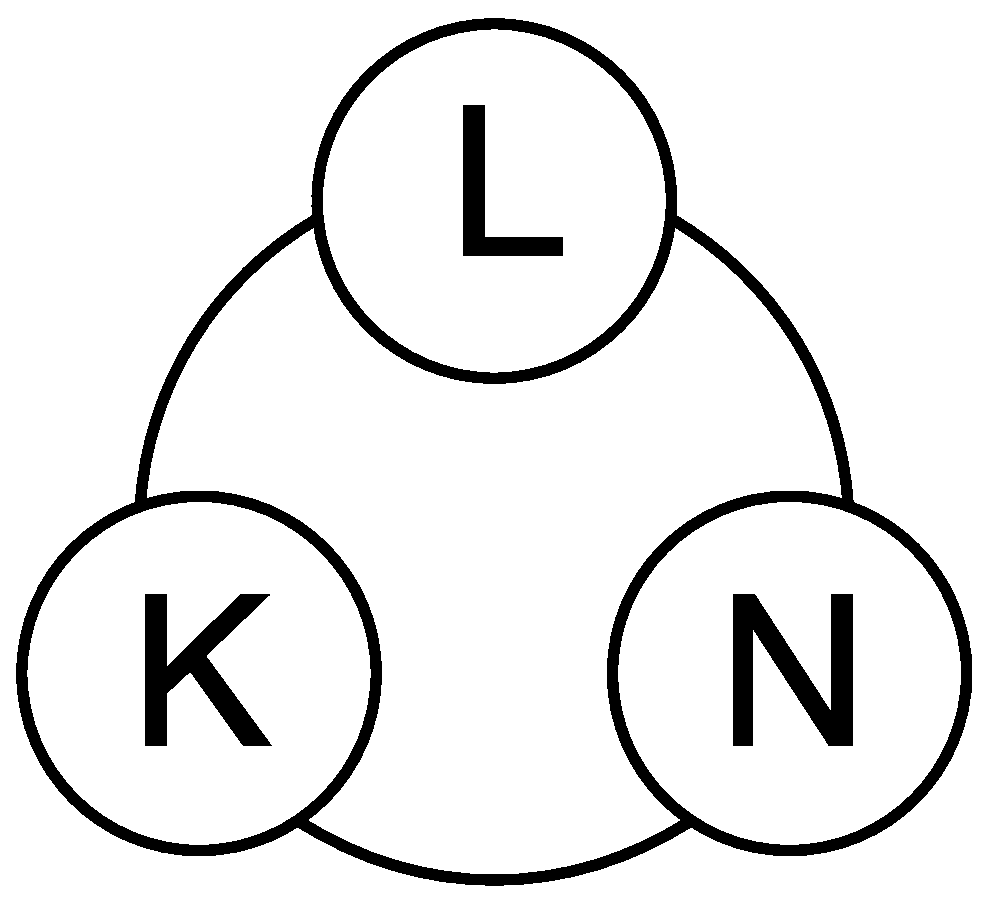
\includegraphics[width=4cm]{LKN_Logo_klein}
  \end{center}

\begin{center} {\sf\bf 
                               \Large  Technische Universität München
                                \smallskip

                               \Large Lehrstuhl für Kommunikationsnetze
                               \smallskip
                              }

                              {\sf \large Prof. Dr.-Ing. Wolfgang Kellerer} 
\end{center}  

\vspace{4cm}

\begin{center}
        {\bf\Huge Bachelor's Thesis} % Studienarbeit, Interdisziplinäres Projekt
\end{center}

\begin{center}
        \settowidth{\baselineskip}{0.4cm}
        {\LARGE 
        AoI-based Scheduling for Networked Control Systems over Gilbert-Elliot Channel 
        }
\end{center}

\vfill         
{\settowidth{\baselineskip}{0.2cm}
\large\begin{tabular}[l]{ll}
Author: & Henry He\\
Supervisor: & M.Sc. Onur Ayan\\
Begin: & 01. June 2020\\
End: & 19. October 2020
\end{tabular}}

%%%%%%%%%%%%%%%%%%%%%%%%%%%%%%%%%%%%%%%%%%%%%%%%%%%%%%%%%%%%

% MAIN PART:
% Independence and License statements
\thispagestyle{plain}


\vspace*{1cm}
With my signature below, I assert that the work in this thesis has been composed by myself independently and no source materials or aids other than those mentioned in the thesis have been used.



\vspace{2cm}

\hspace{1cm}\begin{tabular}{ccc}
\vspace{-0.3cm}München, 19.10.2020 	&\hspace{4cm} 		& \\
\rule{4.5cm}{0.4pt}					&					&\rule{4.5cm}{0.4pt}\\
Place, Date							&					& Signature			
\end{tabular}

           		






\vspace{4cm}
This work is licensed under the Creative Commons Attribution 3.0 Germany License. To view a copy of the license, visit http://creativecommons.org/licenses/by/3.0/de\\

Or\\

Send a letter to Creative Commons, 171 Second Street, Suite 300, San Francisco, California 94105, USA.

\vspace{2cm}



\hspace{1cm}\begin{tabular}{ccc}
\vspace{-0.3cm}München, 19.10.2020 	&\hspace{4cm} 		& \\
\rule{4.5cm}{0.4pt}					&					&\rule{4.5cm}{0.4pt}\\
Place, Date							&					& Signature	
\end{tabular}

% Abstract:
%\setlang{USenglish}
\thispagestyle{plain}

\section*{Abstract}
Many emerging applications to be supported by upcoming 5G networks can be seen
as Networked Control Systems (NCS), i.e., feedback control loops closed over a
communication network. Delay, limited network resources, time-varying channel
conditions are common network-induced challenges which can be tackled by a
scheduler granting medium access efficiently. Age-of-Information (AoI) is a
recently introduced network metric quantifying information freshness at a
receiving network node and is meant to serve as an interface between
communication network and application. AoI has generalized joint design in NCS,
where networking policies have to consider the underlying system dynamics of its
users. It has found successful use-cases in control-aware data scheduling. In
this work, we employ AoI to calculate penalty functions used to derive an
optimal control-aware scheduling strategy. We consider multiple, heterogeneous
NCS sharing a single wireless link with time-varying channel conditions governed
by the Gilbert-Elliot model. We have implemented a channel state dependent
scheduling algorithm and obtained its complexity. However, simulations have
shown that it is not scalable due to high computational costs. Furthermore, we
have investigated possible reasons behind inconsistent behavior of our
scheduling algorithm when simulated on different operating systems. The effect
occurs on Linux, Mac and Windows and results in the scheduler distributing
network resources differently, which leads to varying performance.

% Table of contents:
\tableofcontents  
% Introduction (Einleitung):
\chapter{Introduction}

% This chapter should give a short overview over the whole thesis. It should
% provide background information on the thesis topic, introduce the task
% definition and give a short outlook on the rest of the thesis. 

Development of the upcoming generation of communication networks are largely
driven by changing application demands. Instead of solely focusing on data rate
increase, these networks are envisioned to support machine-type-communications
(MTC) or machine-to-machine communications (M2M), transforming the current
``Internet of Information'' to a ``Internet of Things and Services''. Prominent
applications include vehicular networks, industrial automation, tele-robotics,
smart grids and cyber-physical systems \cite{murray2003future}. From a system
theoretical view, most of these emerging applications fall into the category of
\textit{Networked Control Systems} (NCS), i.e., feedback control loops closed
over a communication network. Each loop consists of a plant, a sensor, measuring
the plant's output, and the respective controller, reacting to the sensor's
data. \\
In a typical NCS scenario, multiple heterogenous NCSs share a wireless
communication medium and compete for network resources to transmit their latest
sensor measurements to the controllers. Medium access is granted by a
centralized scheduler that determines which subset of control loops are allowed
to send their up-to-date state information. In such a setting, the communication
system needs to satisfy different time-critical-requirements of the underlying
control loops, while dealing with problems inherent to the network, such as
random delays, packet losses and time varying channel conditions. These
shortcomings motivate \textit{control-aware} communication protocol design
incorporating prioritization and efficient scheduling of NCSs. Such schedulers
aim to mitigate these network induced challenges, which would otherwise result
in reduced precision of control actions and degraded control quality. Thus,
networking policies need to be designed in a joint fashion by using
\textit{cross-layer} metrics and considering detailed models of feedback control
loops. 

Clearly, the control performance of NCS, i.e., quality of control (QoC), is
tightly coupled with the service provided by the communication network. While
traditionally, performance of network systems are measured by means of delay,
jitter and throughput, these human-oriented metrics do not sufficiently capture
the QoC requirements of heterogeneous NCS applications. Hence, new cross-layer
metrics are needed in control-aware communication protocol design.
Age-of-Information (AoI) is such a relatively new metric that measures the
information freshness at the receiver monitoring a remote process
\cite{kaul2012real} and is used as a cross-layer metric in wireless medium
access protocol design. It is defined as the time elapsed since the generation
of the latest received information. As the name implies, AoI increases linearly
in time for all types of applications and drops upon receiving a new update. AoI
combines packet generation frequency, end-to-end delay, and packet loss in a
single metric. For instance, the absence of information increases AoI on the
controller side regardless of its cause: high delay, packet loss, or a low
information update frequency. As an interface between control application and
communication network, AoI has been widely adopted as an intermediate metric to
calculate control system metrics. 

% While such a setting allows control over large distances, wireless networks
% inevitably introduce random delays, packet losses and time varying channel
% conditions, degrading the control quality. As modern control theory is based on
% the assumption that information are transmitted along perfect communication
% channels, imperfections of the wireless channel or time-critical requirements of
% the underlying control loops impose challenges for both communication and
% control. 

\section*{Problem Statement}
In this work, we aim to develop an optimal scheduling policy addressing a
centralized wireless resource scheduling problem for NCS. We consider multiple
heterogenous feedback control loops sharing a wireless link with time-varying
channel conditions according to the Gilbert-Elliot Model. The deviation of the
real state from the estimated state on the receiver, i.e. controller, is taken
as performance metric. To provide optimal NCS behavior, we utilize AoI-based,
control dependent age-penalties and form scheduling decisions by means of
expected cost minimization. For a similar scenario, \cite{ayan2020aoi} has
proposed an online, centralized scheduling policy that is age-penalty optimal
for a finite horizon $H$. However, similar to most existing works, this solution
assumes a channel with independent and identically distributed (i.i.d) packet
loss. Wireless channels on the other hand are known to generate burst packet
losses/errors, meaning in reality packet losses tend to be correlated. One
simple model capturing correlated losses found in wireless fading channels is
the Gilbert-Elliot Model. We aim to extend the state-of-the-art by combining our
findings of the Gilbert-Elliot Channel Model with the said AoI-based Finite
Horizon scheduler.



% Text Body (Hauptteil)
% Could have multiple chapter-files, e.g.:
\chapter{Background}

% In this chapter, all background necessary to understand the thesis are
% introduced. The level of detail is such that a colleague with similar background
% (no specialist!) is capable of understanding the contribution and impact of the
% thesis. A discussion of state-of-the-art solutions (e.g. literature research) is
% often helpful. Problems of the state-of-the-art are typically discussed and the
% contribution of the thesis is introduced in detail. 

In this chapter, we first present related work on scheduling in NCS scenarios in
Section~(\ref{sec:survey}). Afterwards, we give a short introduction to the
Gilbert-Elliot Channel Model in Section.~(\ref{sec:GE}). 

\section{Related Work} \label{sec:survey}

% Scheduling for NCSs has initially gained research interest from the control
% community, where it has been studied as time-triggered and event-triggered
% control problems \cite{molin2012optimality, molin2014price}. Both papers
% consider optimizations for the steady-state of an NCS with respect to resource
% constraints. While the proposed methods ensure optimal steady-state behavior,
% the network is often assumed control-agnostic and is abstracted. However, 
% the time-varying nature of wireless channels, the trade-offs among different
% control-loops and the coexistence of heterogenous traffic types imply that
% incorporating control metrics in network design can achieve performance benefits
% on the whole system. \\
In communication research a trend towards cross-layer network design has been
shown to be beneficial in NCS settings \cite{park2017wireless}. Error reports
were the first cross-layer metric considered in a centralized resource
scheduling problem with multiple NCS sharing a communication channel
\cite{walsh2001scheduling}. Here, each sensor transmits its estimation error to
the scheduler. The scheduler then allocates free network resources to
sub-systems starting from the ones with maximum-error. In order to account for
underlying time-critical requirements in NCS applications,
\cite{vilgelm2017control} compares control-agnostic scheduling to control-aware
schedulers in a single-hop cellular NCS with varying channel qualities among
control loops. A heuristic scheduling policy is proposed which grants medium
access greedily to the sub-systems with the highest expected error. They have
shown, their control-aware scheduler outperforms an agnostic controller in terms
of maximum throughput with respect to QoC. \cite{vasconcelos2017optimal}
introduces \textit{one-shot} joint scheduling and estimation problem under
resource constraints. Here, a network is shared by multiple sensor and estimator
pairs. Given the probabilistic distributions of individual states, the
centralized scheduler selects a single sensor-estimator pair to transmit. The
authors have shown that it is globally optimal to choose the maximum quadratic
norm as scheduling and mean-value estimation as the estimation strategy. As the
name one-shot suggests, the paper focuses on a single transmission decision and
does not consider application-dependent propagation of estimation error over
multiple time-steps.

This changed in recent years with the introduction of AoI \cite{kaul2012real}.
Due to its ability to connect control and communication layers, AoI has
generalized joint design in NCS. In \cite{kadota2018scheduling}, a multi-user
scenario in which each user is prone to a time-invariant packet loss is
considered. They formulate a discrete-time wireless scheduling problem and show
analytically that the minimum AoI is achieved by updating the user with the
highest AoI. While AoI itself cannot be directly mapped into closed loop control
applications due to AoI evolving linear in time and uniform for all applications
by design. Therefore, \cite{kosta2017age} proposed a non-linear aging concept
called \textit{value-of-information} (VoI) which takes individual application
dynamics into account. \\
AoI based application-dependent age penalties, has first been adopted in
\cite{ayan2019age} for a centralized two-hop uplink and downlink scheduling
problem with heterogenous feedback control loops sharing a cellular network. A
non-linear age dynamic is derived by using AoI as an intermediate metric and
utilizing application specific system parameters. The scheduler accounts for
heterogenous NCS as the proposed age-penalty captures both the propagation of
individual system uncertainties and of the estimation error over time. The
authors show that optimal AoI scheduling results in worse control performance
compared to their proposed greedy VoI scheduling. They extend their findings in
\cite{ayan2020optimal} for multiple heterogeneous NCS but in a single hop
scenario and propose an optimal scheduler that minimizes the discounted
age-penalty over an infinite time horizon. A discount factor takes the
importance of short-term and long-term penalties into consideration, hence,
controlling the scheduler's farsightedness. However, similar to existing
literature, this solution assumes a Bernoulli loss process. To consider
time-varying channel conditions, \cite{ayan2020aoi} assumes i.i.d. packet loss
described by a rectified Gaussian distribution. Although time-varying channel
conditions prevent the calculation of infinite-horizon scheduling policies, they
provide an online scheduling policy that is age-optimal for a finite horizon
using dynamic programming and stochastic optimization. Nonetheless, obtaining
such a policy is computationally expensive and merely optimal for a finite
horizon.

\section{Gilbert-Elliot Model} \label{sec:GE}

In a wireless communication environment, channel errors are bursty, location
dependent, and mobility dependent. These are due to radio propagation
impairments such as shadowing and multi-path fading, as well as interference
from neighboring systems and users. In addition, one must take into account that
users of a wireless network, do not perceive the same channel quality at all
times, where channel quality is considered high when its bit error rate (BER) is
low. Thus, there is one wireless channel (link) between each pair of spatially
distributed nodes (users). 

\begin{figure}[htb]
  \centering
  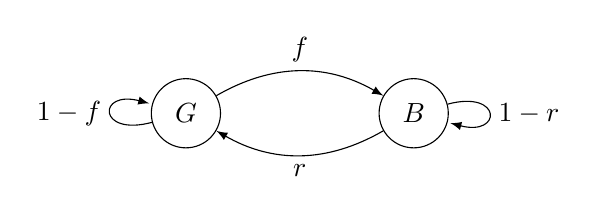
\begin{tikzpicture}[->,>=latex]
  % Create nodes
  \node[state] (G) {$G$};
  \node[state] (B) [right = 2cm of G] {$B$};

  % 
  \path (G) edge [loop left, left] node {$1-f$} (G);
  \path (B) edge [loop right, right] node {$1-r$} (B);
  \path (G) edge [bend left, above] node {$f$} (B);
  \path (B) edge [bend left, below] node {$r$} (G);
\end{tikzpicture}
 
  \caption{The Markov chain for the Gilbert-Elliot Model}
  \label{fig:GE_FSM}
\end{figure}

In the literature, the time-varying quality of a bursty error wireless channel
is commonly modeled using the \textit{Gilbert–Elliot} Model (GE)
\cite{gilbert1960capacity, elliott1963estimates}. It is a widely used stochastic
model for describing bit error processes in transmission channels, where errors
are correlated. There exits several parameterization of this model, but we will
be using the specific Markov chain shown in Fig.~(\ref{fig:GE_FSM}). This model
is a two-state homogenous Markov chain where each of the two states corresponds
to high or low channel quality and is called good state $G$ or bad state $B$,
respectively. Each of them may generate errors as independent events at a state
dependent error rate $p_G$ in the good and $p_B$ in the bad state. As shown in
\cite{hasslinger2008gilbert}, in order to apply the GE model in data loss
processes, we consider the packet reception process as a sequence of bits: 0
stands for a successful arrival of a packet whereas 1 denotes a lost or
corrupted packet.

Let $q(t)$ denote the state at time $t$, then the GE model is defined by the
transition matrix $\boldsymbol{T}$

\begin{equation}
  \label{eq:GE_transition}
  \boldsymbol{T} = 
  \begin{bmatrix}
    1-f & f \\
    r & 1-r \\
  \end{bmatrix},
\end{equation}
\begin{align}
  f &= \Pr[q(t+1) = B \mid q(t) = G] \qquad \textrm{failure rate}, \\
  r &= \Pr[q(t+1) = G \mid q(t) = B] \qquad \textrm{recovery rate},
\end{align}

where $f\in(0,1)$ and $r\in(0,1)$ are the transition probabilities between good
and bad states, respectively. With these definitions, the stationary state
probabilities of the good state $\pi_G$ and the bad state $\pi_B$ exist and can
be defined as follows:

\begin{equation}
  \pi_G = \frac{r}{f+r} \quad \textrm{and} \quad \pi_B = \frac{f}{f+r}
\end{equation}

The stationary state probabilities can be interpreted as the average percentage
of time, in which the channel is in the good or the bad state. Thus, the
\textit{average error probability} is obtained as:

\begin{equation}
  p_E = \pi_G p_G + \pi_B p_B
  \label{eq:avgLoss}
\end{equation}

\subsection{Average Coherence Time}
Another important characteristic defined by the GE model is the mean sojourn
time, i.e., the average duration that the wireless channel stays in a state. In
common NCS scenarios, packet transmissions occur in discrete time slots. Hence,
the channel can only change its state in these time slots and the amount of time
spent in a state is a geometrically distributed random variable $\tau_G$ and
$\tau_B$. Given the state transition probabilities, the mean sojourn times are:

\begin{equation}
  T_G = \E[\tau_G] = \frac{1}{f} \quad \textrm{and} \quad T_B = \E[\tau_B] = \frac{1}{r}
\end{equation}

Table~(\ref{tab:sojournTime}) summarizes sojourn times measurements performed
under different GE parameterization. The measurements resembles the expected
statistical properties of a geometric distribution and confirms our mapping of
state transition probabilities to their corresponding mean sojourn time. Note
that both $f$ and $r$ control the ``burstiness'' of the modeled channel. For
instance, the smaller $r$ is, the longer the channel will stay in the bad state
on average. Hence, longer burst errors are to be expected. Throughout the rest
of the thesis, we will refer $T_G$ and $T_B$ as \textit{average coherence
times}.

\begin{table}[h]
  \begin{center}
  \begin{tabular}{|p{3.5cm}|c|>{\centering\arraybackslash}p{2.05cm}|c|>{\centering\arraybackslash}p{2.05cm}|}
  \hline 
  & \multicolumn{2}{|c|}{\textbf{Time slots in Good}} &
  \multicolumn{2}{|c|}{\textbf{Time slots in Bad}} \\
  \hline
  \textbf{Failure rate} $f$ / \textbf{Recovery rate} $r$ & \textbf{Mean} &
  \textbf{Standard Deviation} & \textbf{Mean}
  & \textbf{Standard Deviation}\\
  \hline \hline
  0.3 & 3.34 & 2.74 & 3.32 & 2.77 \\
  \hline 
  0.1 & 10.0 & 9.56 & 10.0 & 9.29 \\
  \hline 
  0.03 & 33.4 & 32.6 & 34.1 & 34.1 \\
  \hline 
  0.01 & 94.3 & 89.5 & 98.1 & 99.6 \\
  \hline 
  \end{tabular}
  \caption[Measurement of average coherence time in Gilbert-Elliot
  channels]{Measurement of average coherence times for different transition
  probabilities. Note that the state transition probabilities are chosen
  symmetrically for this measurement, i.e. $f=r$}
  \label{tab:sojournTime}
\end{center}
\end{table}

\chapter{Scenario and Problem Statement}

In this chapter, we introduce the considered scenario and give details on the
system, network and control models assumed in Sec.~\ref{sec:system},
Sec.~\ref{sec:network} and Sec.~\ref{sec:control} respectively.
Section~\ref{sec:problem} formulates the wireless resource scheduling problem as
an optimal control problem to be solved by the proposed scheduling scheme.

\section{System Model} \label{sec:system} 

\begin{figure}[htb]
  \centering
  \resizebox*{.8\textwidth}{!}{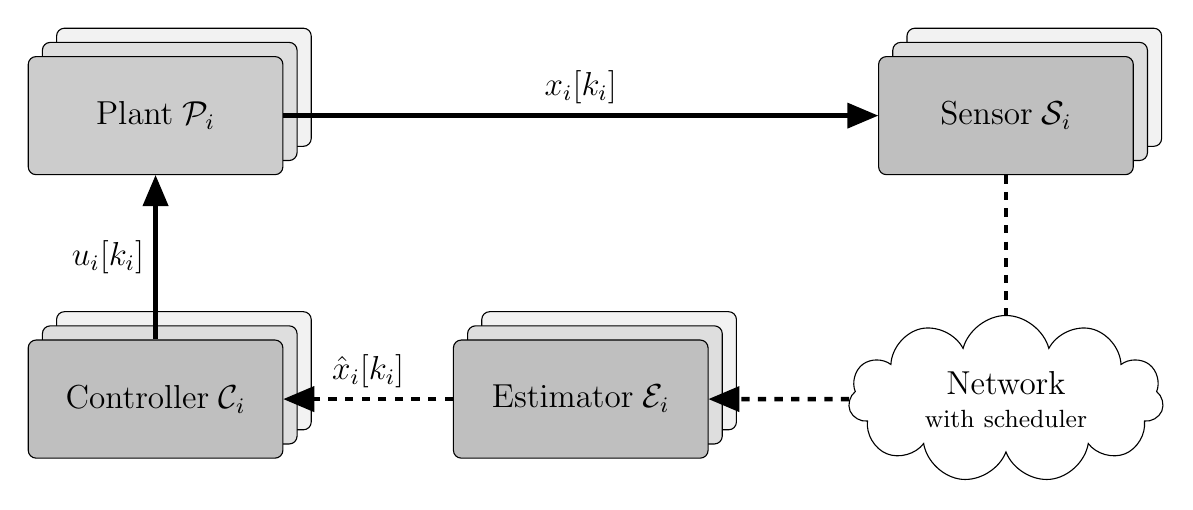
\begin{tikzpicture}[>=latex, scale=0.9]
  \node (plant) at (0.4,6.4) [draw,minimum width=2cm,minimum height=1.5cm, rounded corners=0.1cm, text width=3cm, align=center, fill=mylightestgray] {};
  
  \node (plant) at (0.2,6.2) [draw,minimum width=2cm,minimum height=1.5cm, rounded corners=0.1cm, text width=3cm, align=center, fill=mylightergray] {};
  
  % Plant
  \node (plant) at (0,6) [draw,minimum width=2cm,minimum height=1.5cm, rounded corners=0.1cm, text width=3cm, align=center, fill=mygray] {\large{Plant $\mathcal{P}_i$}};
  
  
  % Sensor 
  \node (sensor) at (12.4,6.4) [draw,minimum width=2cm,minimum height=1.5cm, rounded corners=0.1cm, text width=3cm, align=center, fill=mylightestgray] {};
  
  \node (sensor) at (12.2,6.2) [draw,minimum width=2cm,minimum height=1.5cm, rounded corners=0.1cm, text width=3cm, align=center, fill=mylightergray] {};
  
  \node (sensor) at (12,6) [draw,minimum width=2cm,minimum height=1.5cm, rounded corners=0.1cm, text width=3cm, align=center, fill=lightgray] {\large{Sensor $\mathcal{S}_i$}};
  
  %Estimator
  \node (estimator) at (6.4,2.4) [draw,minimum width=2cm,minimum height=1.5cm, rounded corners=0.1cm, text width=3cm, align=center, fill=mylightestgray] {\large{Estimator $\mathcal{E}_i$}};

  \node (estimator) at (6.2,2.2) [draw,minimum width=2cm,minimum height=1.5cm, rounded corners=0.1cm, text width=3cm, align=center, fill=mylightergray] {\large{Estimator $\mathcal{E}_i$}};

  \node (estimator) at (6,2) [draw,minimum width=2cm,minimum height=1.5cm, rounded corners=0.1cm, text width=3cm, align=center, fill=lightgray] {\large{Estimator $\mathcal{E}_i$}};


  % Controller
  \node (controller) at (0.4,2.4) [draw,minimum width=2cm,minimum height=1.5cm, rounded corners=0.1cm, text width=3cm, align=center, fill=mylightestgray] {};
  
  \node (controller) at (0.2,2.2) [draw,minimum width=2cm,minimum height=1.5cm, rounded corners=0.1cm, text width=3cm, align=center, fill=mylightergray] {};
  
  \node (controller) at (0,2) [draw,minimum width=2cm,minimum height=1.5cm, rounded corners=0.1cm, text width=3cm, align=center, fill=lightgray] {\large{Controller $\mathcal{C}_i$}};
  
  
  % Network Cloud
  \node[cloud, cloud puffs=11, cloud ignores aspect, minimum width=2cm, minimum height=1.5, text width=2.5cm, align=center, draw] (cloud) at (12, 2) {\large {Network \\} \small{with scheduler}};
  
  % C-to-P arrow
  \draw[arrows=-triangle 45,black, ultra thick] (controller.north) -- node[pos=0.5, left] {\large $u_i[k_i]$} (plant.south);
  
  % P-to-S arrow
  \draw[arrows=-triangle 45,black, ultra thick] (plant.east) -- node[pos=0.5, above] {\large $x_i[k_i]$} (sensor.west);
  
  % P-to-Cloud arrow
  \draw[black, dashed, ultra thick] (sensor.south) -- node[] {} (cloud.north);
  
  % Cloud-to-E arrow
  \draw[arrows=-triangle 45,black, dashed, ultra thick] (cloud.west) -- node[pos=0.5, above] {} (estimator.east);

  % E-to-C arrow
  \draw[arrows=-triangle 45,black, dashed, ultra thick] (estimator.west) -- node[pos=0.5, above] {\large $\hat{x}_i[k_i]$} (controller.east);
  
  \end{tikzpicture}
} 
  \caption[Scheme of $N$ sub-systems sharing a wireless communication
  medium]{Considered scenario with $N$ heterogeneous LTI networked control
  systems. Solid lines indicate ideal controller-to-plant and plant-to-sensor
  links. Sensor-to-controller links are closed over a shared wireless channel.
  Medium access is granted centrally by a scheduler. Note that $k_i$ refers to
  the sampling period a sub-system $i$ is in.}
  \label{fig:scenario}
\end{figure}

We consider $N$ independent, linear time-invariant (LTI) control systems sharing
a wireless communication network. Each individual sub-system $i$ consists of a
plant $\plant$, a sensor $\sensor$ and a controller $\controller$ with an
estimator $\estimator$. Every sensor $\sensor$ measures the output of the plant
periodically and sends the latest sample to $\controller$. On the controller
side, $\estimator$ estimates the current plant state based on the latest
received information. Estimated state is then used by $\controller$ to calculate
the next control input. Each controller-plant pair is assumed to be connected
through an ideal link, while the sensor is operating remotely over the shared
wireless channel as illustrated in Fig.~\ref{fig:scenario}.

\section{Network Model} \label{sec:network} 

In our scenario we consider time to progress in discrete time slots and use $t
\in \mathbb{N}$ to index them. Sensors $\sensor$ transmit state information over
a wireless medium in packets containing a single measurement. We assume
simplified packet transmission, where each packet sent in slot $t$ is received
within the same slot and packets are neither acknowledged nor retransmitted to
reduce protocol overhead. Medium access is granted by a centralized entity
called \textit{scheduler}, which at each time slot $t$, decides which sub-system
is allowed to transmit its latest plant measurement. Moreover, only a single
transmission resource is allocated within a single time slot. Let $\delta_i(t)
\in \left\{0,1\right\}$ denote the scheduler decision variable being
$\delta_i(t)=1$ if the sub-system $i$ is allowed to transmit in slot $t$ and
$\delta_i(t)=0$ otherwise. Then the following holds for all time slots:

\begin{equation}
  \sum_{i=1}^{N}{\delta_i(t) \leq 1 \quad, \forall t}
\end{equation}

We consider a bursty GE channel where the link quality between each
sensor-controller pair is time and channel state dependent. (See
Sec.~{\ref{sec:GE}}) Each link is prone to its own channel state $q_i(t)$ which
determines the probability $p_i(t) \in \left\{p_G,p_B\right\}$ a packet is lost.
That is, if we define a success indicator variable $\gamma_i(t)\in\{0,1\}$
representing a failed $\gamma_i(t)=0$ or a successful $\gamma_i(t)=1$ packet
reception, then the probabilities for a success and failure are given by
$\Pr[\gamma_i(t)=1 \mid \delta_i(t)=1] = 1-p_i(t)$ and  $\Pr[\gamma_i(t)=0 \mid
\delta_i(t)=1] = p_i(t)$, respectively. \\ 
% For the sake of completeness, note that $\Pr[\gamma_i[t]=1 \mid \delta_i[t]=0]
% = 0$ and $\Pr[\gamma_i[t]=0 \mid \delta_i[t]=0] = 1$. 
The control-aware scheduler is assumed to be able to measure the instantaneous
link quality for each sensor-estimator pair, thus knows the current loss
probabilities $p_i(t)$. Further, the scheduler will make decisions by
considering control and network behaviors. The network state is comprised of
variables defined in the following.

\subsection{Network state}

Packets are generated periodically at $\sensor$ every $D_i \in \mathbb{Z}^+$
slots. We refer to the generation of a packet as a \textit{sampling event} and
the time between two consecutive sampling events as the \textit{sampling
period}. Let $t_{i,o} \sim \mathcal{U}[0, D_i)$ denote the initial sampling
event of sub-system $i$, then the set of slots in which a sampling event occurs
are:

\begin{equation}
  \mathcal{G}_i \triangleq \lbrace t_{i,o}, \; t_{i,o} + D_{i}, \; t_{i,o} + 2 D_{i}, \; \dots \rbrace 
\end{equation}

As $t_{i,o}$ is a uniformly distributed random variable and not necessarily
equal for each sub-system, we allow sampling to operate in a non-synchronized
fashion. 

\begin{figure}[htb]
  \centering
  \resizebox*{.6\textwidth}{!}{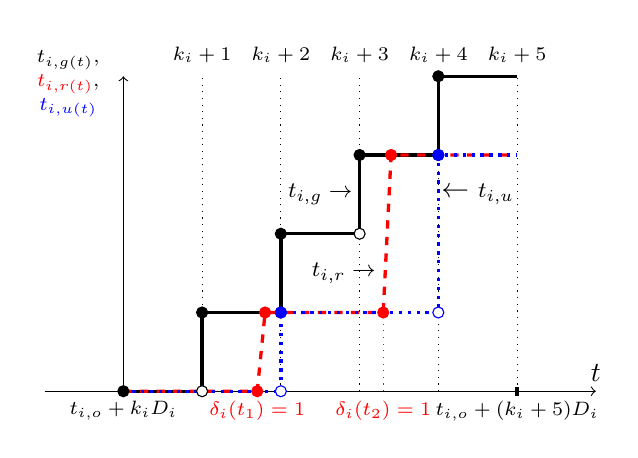
\begin{tikzpicture}

% horizontal axis
\draw[->] (-1,0) -- (6,0) node[anchor=south] {$t$};
% labels
\draw	(0,4.5) node[anchor=east] {}
		(1,4.5) node[anchor=north] {\scriptsize$k_i+1$}
		(2,4.5) node[anchor=north] {\scriptsize$k_i+2$}
		(3,4.5) node[anchor=north] {\scriptsize$k_i+3$}
		(4,4.5) node[anchor=north] {\scriptsize$k_i+4$}
		(5,4.5) node[anchor=north] {\scriptsize$k_i+5$}
		(0,-0.0) node[anchor=north]
		{\scriptsize$t_{i,o} + k_i D_i$}
		(5,-0.0) node[anchor=north]
		{\scriptsize$t_{i,o}+(k_i+5)D_i$}
		(1.7,-0.0) node[anchor=north] {\color{red}\scriptsize$\delta_i(t_1)=1$}
		(3.3,-0.0) node[anchor=north] {\color{red}\scriptsize$\delta_i(t_2)=1$};

\node[] at (-0.7, 4.2) {\scriptsize$t_{i,g(t)}$,};
\node[] at (-0.7, 3.9) {\color{red}{\scriptsize$t_{i,r(t)}$}\color{black}{\scriptsize,}};
\node[] at (-0.7, 3.6) {\color{blue}{\scriptsize$t_{i,u(t)}$}};

\draw[very thick, black] (5,-0.06) --  (5,+0.06);
	
% vertical axis
\draw[->] (0,0) -- (0,4) node[anchor=east] {};
% vertical ticks
\draw[dotted] (1,0) -- (1,4);
\draw[dotted] (2,0) -- (2,4);
\draw[dotted] (3,0) -- (3,4);
\draw[dotted] (4,0) -- (4,4);
\draw[dotted] (5,0) -- (5,4);
\draw[dotted,red] (3.3,0) -- (3.3,1);

% Delta 1
%\draw[very thick, black, solid] (0,1) -- (1,1);
%\draw[very thick, black, solid] (1,0) -- (2,0);
%\draw[very thick, black, solid] (2,1) -- (3,1);
%\draw[very thick, black, solid] (3,2) -- (4,2);
%\draw[very thick, black, solid] (0,1) -- (1,1);
%\draw[very thick, black, solid] (0,1) -- (1,1);
\draw[very thick, black, solid] (0,0) --  (1,0) -- (1,1) -- (2,1) -- (2,2) -- (3,2) --  (3,3) -- (4,3) -- (4,4)-- (5,4);

\draw[very thick, red, dashed] (0,0) --  (1.7,0) -- (1.8,1) -- (3.3,1) -- (3.4,3) -- (5,3);

\draw[very thick, blue, dotted] (0,0) --  (2,0) -- (2,1) -- (4,1) -- (4,3) -- (5,3);

%\draw (-.7, 1) node {\scriptsize$\Delta[k-1]$}; %label
\draw (2.5, 2.5) node { \footnotesize$t_{i,g}\rightarrow$};

\draw (2.8, 1.5) node { \footnotesize$t_{i,r}\rightarrow$};

\draw (4.5, 2.5) node { $\leftarrow\,\,$\footnotesize$t_{i,u}$};



\node[circle,draw=black, fill=white, inner sep=0pt,minimum size=4pt] (b) at (1,0) {};
\node[circle,draw=black, fill=white, inner sep=0pt,minimum size=4pt] (b) at (2,1) {};
\node[circle,draw=black, fill=white, inner sep=0pt,minimum size=4pt] (b) at (3,2) {};
\node[circle,draw=black, fill=white, inner sep=0pt,minimum size=4pt] (b) at (4,3) {};


\node[circle,draw=black, fill=black, inner sep=0pt,minimum size=4pt] (b) at (0,0) {};
\node[circle,draw=black, fill=black, inner sep=0pt,minimum size=4pt] (b) at (1,1) {};
\node[circle,draw=black, fill=black, inner sep=0pt,minimum size=4pt] (b) at (2,2) {};
\node[circle,draw=black, fill=black, inner sep=0pt,minimum size=4pt] (b) at (3,3) {};
\node[circle,draw=black, fill=black, inner sep=0pt,minimum size=4pt] (b) at (4,4) {};
%\node[circle,draw=black, fill=black, inner sep=0pt,minimum size=4pt] (b) at (5,4) {};

\node[circle,draw=blue, fill=white, inner sep=0pt,minimum size=4pt] (b) at (2,0) {};
\node[circle,draw=blue, fill=white, inner sep=0pt,minimum size=4pt] (b) at (4,1) {};



\node[circle,draw=blue, fill=blue, inner sep=0pt,minimum size=4pt] (b) at (2,1) {};
\node[circle,draw=blue, fill=blue, inner sep=0pt,minimum size=4pt] (b) at (4,3) {};


\node[circle,draw=red, fill=red, inner sep=0pt,minimum size=4pt] (b) at (1.7,0) {};
\node[circle,draw=red, fill=red, inner sep=0pt,minimum size=4pt] (b) at (3.3,1) {};



\node[circle,draw=red, fill=red, inner sep=0pt,minimum size=4pt] (b) at (1.8,1) {};
\node[circle,draw=red, fill=red, inner sep=0pt,minimum size=4pt] (b) at (3.4,3) {};


\end{tikzpicture}
} 

  \caption[Example evolution of generation time $t_{i,g}$, received time
  $t_{i,r}$ and update time $t_{i,u}$]{Evolution of generation time
  $t_{i,g}(t)$, received time $t_{i,r}(t)$ and the update time $t_{i,u}(t)$.
  $t_{i,g}(t)$ and $t_{i,u}(t)$ update their values periodically every $D_i$
  slots, while $t_{i,r}(t)$ can progress asynchronously. Two exemplary
  successful packet transmission $\delta_i(t_{1,2})=1$ are illustrated.}
  \label{fig:ageplot}
\end{figure}  

The controller does not benefit from receiving an older plant measurement, if it
has already received a more recent measurement \cite{costa2016age}. Therefore,
sensors replace their packet in the transmit buffer with a more recent
measurement whenever a newer update arrives. We define a variable $t_{i,g}(t)$
that denotes the time the packet waiting for transmission at $\sensor$ was
generated. Since packets are solely generated during a sampling event, $t \in
\mathcal{G}_i$ are the only possible values $t_{i,g}$ can have. Thus, $t_{i,g}$
evolves as follows:

\begin{equation}
  t_{i,g}(t+1) =
  \begin{cases}
  t+1 & \text{, if } t+1 \in \mathcal{G}_i \\
  t_{i,g}(t) & \text{, otherwise}	
  \end{cases}
\end{equation}

We further define $t_{i,r}(t)$ as the generation time of the newest packet
received by $\controller$ until time $t$:

\begin{equation}
  t_{i, r}(t+1) =
  \begin{cases}
  t_{i, g}(t) & \text{, if } \delta_i(t) \cdot \gamma_i(t) = 1 \\
  t_{i, r}(t) & \text{, otherwise}	
  \end{cases}
\end{equation}

Fig.~\ref{fig:ageplot} shows an exemplary evolution of $t_{i,g}$, along with how
${t_{i,r}(t+1)}$ and $t_{i,g}(t)$ are correlated to each other after two
successful updates. Generation time $t_{i,g}$ demonstrates a discrete staircase
behavior at $t \in \mathcal{G}_i$, while received time $t_{i,r}$ can take new
values at any slot $t \in \mathbb{N}$ subject to the indication variables
$\delta_i$ and $\gamma_i$.

\section{Control Model} \label{sec:control}

The system of the $i$-th plant $\plant$ is considered to evolve by the following
LTI model over discrete time:

\begin{equation}
  \label{eq:discretemodel}
  \boldsymbol{x}_i[k_i+1] = \boldsymbol{A}_i \boldsymbol{x}_i[k_i] + \boldsymbol{B}_i \boldsymbol{u}_i[k_i] + \boldsymbol{w}_i[k_i]
\end{equation}

with time-invariant system matrix $\boldsymbol{A}_i \in \mathbb{R}^{n_i\times
n_i}$ and input matrix $\boldsymbol{B}_i \in \mathbb{R}^{n_i\times m_i}$. System
noise is denoted by $\boldsymbol{w}_i \in \mathbb{R}^{n_i}$ which is
characterized by a multi-variate Gaussian distribution with zero mean and
diagonal covariance matrix $\mathbf{\Sigma}_i \in \mathbb{R}^{n_i}$, i.e.,
$\boldsymbol{w}_i \sim \mathcal{N}(\mathbf{0}, \mathbf{\Sigma}_i)$. We assume
the sub-systems to operate slower than the network. In other words, the plant
state changes only after each sampling event and remains constant until the next
one. Thus, the discrete dynamics of sub-systems as described in
Eq.~\eqref{eq:discretemodel} is indexed by a different time variable $k_i$. It
indicates in which sampling period a sub-system currently is and can be obtained
at any time slot $t$ with:

\begin{equation}
  \label{eq:k_map}
	k_i(t) = \floor{\frac{t - t_{i,o}}{D_i}}
\end{equation}

In addition, $\boldsymbol{x}_i[k_i] \in \mathbb{R}^{n_i}$ and
$\boldsymbol{u}_i[k_i] \in \mathbb{R}^{m_i}$ represent the system state and
control input in sampling period $k_i$, respectively. At the beginning of each
sampling period $k_i$, i.e., at $t=t_{i,o}+k_iD_i$, the controller $\controller$
calculates $\boldsymbol{u}_i[k]$ given the available observation history and
actuates $\plant$ with the obtained control input within the same sampling
period. As a result, any packet arriving in sampling period $k_i$ after
$\boldsymbol{u}_i[k_i]$ is calculated, will be queued until it is first utilized
in the next control input $\boldsymbol{u}_i[k_i+1]$. To capture the
aforementioned update delay of successfully received packets, we introduce
$t_{i,u}(t)$ as the generation time of the latest utilized packet by
$\controller$:

\begin{equation}
  \label{eq:t_u}
  t_{i, u}(t+1) =
  \begin{cases}
  t_{i, r}(t+1) & \text{, if } t+1 \in \mathcal{G}_i \\ 
  t_{i, u}(t) & \text{, otherwise}	
  \end{cases} 
\end{equation}

Time dynamics of $t_{i,u}$ is seen in Fig.~\ref{fig:ageplot} where it takes the
value of $t_{i,r}$ at the end of a control system period $t \in \mathcal{G}_i$.

\subsection{Age-of-Information Model}
The discrete-time model allows for communication and control to evolve in
different time steps. Particularly, changes in our control model occur at
sampling events. Thus, in a control application's point of view, plant
observations included in packets age only every $D_i$ slots. Information
staleness is then expressed in multiples of $D_i$. Therefore, we AoI is defined
as the number of sampling periods elapsed since the acquisition of the latest
received system state at $\controller$, which can be determined at any slot $t$
as:

\begin{equation}
  \label{eq:aoi}
  \Delta_i(t) = \ceil{\dfrac{t - t_{i,u}(t)}{D_{i}}} 
\end{equation}

It should be noted that since packets arrive at least one slot delayed, a packet
received in a sampling period can never be utilized immediately in the same
sampling period. Hence, the minimum AoI in our scenario is one, i.e.,
$\Delta_i(t) \ge 1,\forall i,t$.

\subsection{Remote Estimation and Control Law}
In order to compensate for packet drops or delays caused by the network, each
controller $\controller$ employs a Kalman-like state estimator $\estimator$
based on the following assumptions:

\begin{theorem}
  The controller $\controller$ and its estimator $\estimator$ are aware of the
  control system parameters $\boldsymbol{A}_i, \boldsymbol{B}_i$ and
  $\boldsymbol{w}_i$.
\end{theorem}

\begin{theorem}
  $t_{i,o}, D_i$ and $t$ are also known by the controller. 
\end{theorem}

Assumption 1 is motivated by the time-invariant nature of the sub-system's
dynamics. Assumption 2 allows the estimation-based controller to map any $t$ to
$k_i$ by using Eq.~\eqref{eq:k_map}. As a result, the controller can determine
the AoI of its most up-to-date plant state information $\boldsymbol{x_i}[k_i -
\Delta_i[k_i]]$ which is $\Delta_i[k_i]$ sampling periods old.

Combining our assumptions, each estimator $\estimator$ predicts the current
plant state by means of a conditional expectation, i.e.,
$\hat{\boldsymbol{x}}_i[k_i] = \E\left[\boldsymbol{x}_i[k_i] \mid \Delta_i[k_i],
\boldsymbol{x}_i[k_i-\Delta_i] \right]$. We leverage the results from
\cite{ayan2019age}, stating that the optimal estimation which minimizes the
mean-squared error is obtained by:

\begin{equation}
  \label{eq:estimatedstate}
    \boldsymbol{\hat{x}}_i[k_i] = \boldsymbol{A}_i^{\Delta_i[k_i]} \,  \boldsymbol{x}_i[k_i - \Delta_i[k_i]] + \sum_{q=1}^{\Delta_i[k_i]} \boldsymbol{A}_i^{q - 1} \, \boldsymbol{B}_i \, \boldsymbol{u}_i [k_i - q].
\end{equation}

To perform this estimation, $\estimator$ has to keep track of the last
$\Delta_i[k_i]$ control inputs. However, this information is generated locally
and thus already available to $\estimator$. Further, with
Eq.~\eqref{eq:discretemodel} and \eqref{eq:estimatedstate} the estimation error
$\boldsymbol{e}_i[k_i]$ is obtained as:

\begin{equation}
  \boldsymbol{e}_i[k_i] \triangleq \boldsymbol{x}_i[k_i] - \boldsymbol{\hat{x}}_i[k_i] = \sum_{q=1}^{\Delta_i[k_i]} \boldsymbol{A}_i^{q-1} \, \boldsymbol{w}_i[k_i - q].
\end{equation}

By taking the euclidean norm of $\boldsymbol{e}_i[k_i]$ the expected mean
squared error (MSE) at $\controller$ is given as:

\begin{align}
  \label{eq:estimationerror}
  \E \left[ \left(\boldsymbol{e}_i[k_i]\right)^T \, \boldsymbol{e}_i[k_i]\right] & = \sum_{r=1}^{\Delta_i[k_i] - 1} \tr \left( \left(\boldsymbol{A}_i^T\right)^r  \left(\boldsymbol{A}_i \right)^r \boldsymbol{\Sigma}_i \right) \\ \nonumber
  & \triangleq g(\Delta_i[k_i]).
\end{align}

It is important to note that Eq.~\eqref{eq:estimationerror} only depends on
$\Delta_i[k_i]$ and is independent from the actual system state
$\boldsymbol{x}_i[k_i]$. This would not be true in the case of time-variant
control systems. Here, we define $g(\Delta_i[k_i])$ as our AoI-based age-penalty
that penalizes high estimation errors and will be subject to minimization in the
scheduling problem.

After obtaining a state estimation, it is utilized in calculating the control
input according to the following control law:

\begin{equation}
  \label{eq:controllaw}
  \boldsymbol{u}_i[k_i] = - \boldsymbol{L}_i^* \,\boldsymbol{\hat{x}}_i[k_i],
\end{equation}

where $\boldsymbol{L}_i^* \in \mathbb{R}^{m_i \times n_i}$ is the feedback gain
matrix. 

% $\boldsymbol{L}^*_i$ is obtained from:
% \begin{equation}
%   \label{eq:optimalgain}
%   \boldsymbol{L}_i^* = \left(\boldsymbol{R}_i + \boldsymbol{B}_i^T \boldsymbol{P}_i \boldsymbol{B}_i \right)^{-1} \boldsymbol{B}_i^T \boldsymbol{P}_i \boldsymbol{A}_i,
% \end{equation}

% which solves the discrete time algebraic Riccati equation:
% \begin{equation}
%   \label{eq:riccati}
%   \boldsymbol{P}_i = \boldsymbol{Q}_{i} + \boldsymbol{A}_i^T \left(\boldsymbol{P}_i - \boldsymbol{P}_i \boldsymbol{B}_i ( \boldsymbol{R}_{i} + \boldsymbol{B}_i^T \boldsymbol{P}_i \boldsymbol{B}_i)^{- 1} \boldsymbol{B}_i^T \boldsymbol{P}_i \right) \boldsymbol{A}_i.
% \end{equation}

% $\boldsymbol{Q}_{i}$ and $\boldsymbol{R}_{i}$ are weighting matrices of
% appropriate size that penalize the state and control inputs in the infinite
% horizon, \textit{Linear-quadratic-Gaussian} (LQG) cost function $F_i$:

% \begin{equation}
%   F_i = \dfrac{1}{K} \limsup_{K \rightarrow \infty} \sum_{k_i=0}^{K-1} (\boldsymbol{x}_i[k_i])^T \boldsymbol{Q}_i \boldsymbol{x}_i[k_i] +  (\boldsymbol{u}_i[k_i])^T \boldsymbol{R}_i \boldsymbol{u}_i[k_i]. 
% \end{equation}

% One can interpret $F_i$ as an indicator of control performance. The lower $F_i$
% is, the higher is the \textit{quality of control}.

\section{Scheduling Problem Formulation} \label{sec:problem} 

From Eq.~\eqref{eq:estimationerror} it is evident, that expected estimation
performance is controlled by the AoI of sub-systems. By scheduling a certain
control application, information with low $\Delta_i[k_i]$ is provided to its
estimator, resulting in low age-penalties. In chapter~\ref{ch:scheduler}we will
derive a scheduler whose aim is to minimizes the total expected cost and thereby
providing good overall estimation accuracy. Let $\mu(t')\in\left\{\varnothing,
1, \dots,N \right\}$ denote the scheduling decision at slot $t'$, which indexes
the sub-system that is granted medium access. Note that $\mu(t')=i$ implies
$\delta_i(t')=1$. We are interested in finding scheduling policies $\pi$
consisting of a sequence of scheduling decisions $\mu(t')$ for the next $H \in
\mathbb{Z}^+$ slots:

\begin{equation}
  \pi=\left\{ \mu(t), \mu(t+1), \dots, \mu(t+H-1) \right\}
\end{equation}

Such policies will be called \textit{admissible}. $H$ is the \textit{finite
horizon} parameter that defines how many future slots are being considered by
$\pi$. Thus, $H$ governs the ``farsightedness'' of the proposed scheduler.

We consider the wireless resource scheduling problem as a general problem of
decision under stochastic uncertainty \cite{bertsekas1995dynamic}. Such a
problem has two principal features. An underlying discrete-time dynamic system
and an \textit{additive} cost function $J$ that is dependent on the system's
state. In our case, the dynamic system is the wireless network whose system
state $\boldsymbol{s} \in \mathbb{Z}^{4\cdot N}$ we define as:

\begin{equation}
  \boldsymbol{s}(t) \triangleq \left[\boldsymbol{t}_g(t) \quad \boldsymbol{t}_r(t) \quad \boldsymbol{t}_u(t) \quad \boldsymbol{q}(t)\right]^T, 
\end{equation}   
with: 
\begin{align}
  \boldsymbol{t}_g(t) &\triangleq \left[ t_{1,g}(t) ~ \dots ~ t_{N,g}(t) \right]^T ,\\
  \boldsymbol{t}_r(t) &\triangleq \left[ t_{1,r}(t) ~ \dots ~ t_{N,r}(t) \right]^T ,\\
  \boldsymbol{t}_u(t) &\triangleq \left[ t_{1,u}(t) ~ \dots ~ t_{N,u}(t) \right]^T ,\\
  \boldsymbol{q}(t) &\triangleq \left[ q_1(t) ~ \dots ~ q_N(t) \right].
\end{align}  

The evolution of the network's state depends on the outcome of packet
transmissions over the wireless network. Otherwise speaking, network dynamics
are affected by random packet loss. As a consequence, given a ``control'' input
$\mu(t)$ not only one but multiple next network states are possible. Each of
these transitions follow a probability distribution $Pr\left[\cdot\mid\mu(t),
\boldsymbol{s}(t) \right]$. While possible next states are under the influence
of made scheduling decisions, their corresponding transition probability is a
function of $p_i(t)$ and $f,r$ defined by the GE model. Particularly, given a
state $\boldsymbol{s}(t)$ and a scheduling decision $\mu(t)=i$, the transition
probability to a possible next state $\boldsymbol{s'}$ is expressed by:

\begin{equation}
  \label{eq:transition}
  \Pr \left[ \boldsymbol{s}(t+1)=\boldsymbol{s}' \mid \mu(t)=i,\boldsymbol{s}(t)
  \right] \in \left\{ p \cdot q \mid p\in\mathcal{L},q\in\mathcal{T} \right\},
\end{equation}

where $\mathcal{L}=\left\{p_G,p_B\right\}^N$ are GE channel state dependent loss
probabilities and $\mathcal{T}=\left\{f,r\right\}$ the failure and recovery
rates defined in the Markov chain's stochastic transition matrix in
Eq.~\eqref{eq:GE_transition}.

Consider $C(\boldsymbol{s}(t))$ as state cost incurred by being in
$\boldsymbol{s}(t)$ at time $t$. To penalize high estimation errors, we define
$C(\boldsymbol{s}(t))$ as the total expected MSE over all sub-systems:

\begin{equation}
  \label{eq:gfunction}
  C(\boldsymbol{s}(t)) =  \sum_{i=1}^{N}  g(\Delta_i[k_i(t)]),
\end{equation}

where $g(\Delta_i[k_i(t)])$ is the expected estimation error of a single
sub-system as defined in Eq.~\eqref{eq:estimationerror}. 

The cost function $J$ is \textit{additive} over time in the sense that cost
acquired at time $t$, i.e., $C(\boldsymbol{s}(t))$, accumulates over time.
Meaning that the total expected finite horizon cost $J_{\pi}(\boldsymbol{s}(t))$
for any initial state $\boldsymbol{s}(t)$ and horizon $H$ is defined as:

\begin{equation}
  \label{eq:horizoncost}	
  J_\pi(\boldsymbol{s}(t)) \triangleq \E_\pi \left[ \sum_{t' = t }^{t + H} C(\boldsymbol{s}(t')) \right] 
\end{equation}

Note that since network transmissions occur stochastically,
$C(\boldsymbol{s}(t))$ is a random variable and therefore we consider the
expectation of the total cost. Further, as feasible next states depend on the
scheduling decisions $\mu(t')$, the subscript $\pi$ in $J_\pi$ and $\E_\pi$
indicate that Eq.~\eqref{eq:horizoncost} quantifies the expected cost when the
scheduling policy $\pi = \{ \mu(t), {\mu(t+1)}, \dots, \mu(t+H-1) \}$ is applied
over the horizon $H$. Our goal is to find the optimal policy $\pi^*$, such that
$J_{\pi^*}(\boldsymbol{s}(t))$ is minimal:

\begin{equation}
\label{eq:minimizationproblem}
	J_{\pi^*}(\boldsymbol{s}(t)) = \min_{\pi \in \Pi} J_\pi (\boldsymbol{s}(t)) = J^*(\boldsymbol{s}(t)),
\end{equation}

where $\Pi$ is the set of all admissible policies. In addition, to only allow
sub-systems with new information to transmit, we reduce the set of possible
actions given the network state $\boldsymbol{s}(t)$ at each time slot $t$ to:

\begin{gather}
  \label{eq:admissibleactions}
  \mathcal{M}(\boldsymbol{s}(t)) = \{\varnothing\} \cup \{i : t_{i,g}(t) > t_{i,r}(t) \}, \\
  \mu(t) \in \mathcal{M}(\boldsymbol{s}(t))
\end{gather}

This allows us to confine our search for an optimal scheduling policy within
this smaller set. Together with the search space, the scheduler's complexity is
also reduced without losing optimality. Throughout the remaining thesis, we
refer to the minimization problem in Eq.~\eqref{eq:minimizationproblem} as the
$H$-stage problem and drop the subscript $\pi$ for brevity.

\chapter{Scheduler Design}

In this chapter, we develop an online scheduling scheme that solves the $H$
stage-problem by employing Dynamic Programming and Stochastic Optimization.
First, Sec. \ref{sec:fhscheduler} summarizes the state-of-the-art Finite Horizon
Scheduler which our proposed scheduler is based on. We extend it to be
applicable in NCS scenarios with Gilbert-Elliot channels and give a short
complexity analysis in Sec. \ref{sec:gescheduler}.

\section{Finite Horizon Scheduler} \label{sec:fhscheduler}

In \cite{ayan2020aoi} a \textit{finite horizon scheduler (FHS)} is proposed
which takes optimal scheduling decisions for the next $H$ transmission slots. In
contrast to our scenario, independent losses drawn from a normal distribution
are considered, not accounting for GE channel state transitions, i.e.,
$\boldsymbol{s}(t) = \left[\boldsymbol{t}_g(t) \quad \boldsymbol{t}_r(t) \quad
\boldsymbol{t}_u(t) \right]^T$. This also means, that network state transitions
are solely dependent on packet loss probabilities.  

FHS solves the formulated $H$-stage problem by applying the Dynamic Programming
Algorithm (DP) \cite{bertsekas1995dynamic}. The fundamental idea behind DP is to
break down a complicated problem into simpler subproblems, obtaining the
solution by iteratively combining solutions of small subproblems in a
bottom-up-approach. This is motivated by the \textit{principle of optimality},
which intuitively states that every optimal policy consists only of optimal sub
policies. That is, assume $\pi^* = \{\mu^*(t), \mu^*(t+1), \dots, \mu^*(t+H-1)
\}$ to be an optimal policy for the $H$-stage problem. For the subproblem
whereby we are at at time $i>t$ and wish to minimize the \textit{cost-to-go}
from $\boldsymbol{s}(i)$ at time $i$ to time $H$, i.e.,

\begin{equation}
  \label{eq:costtogo}
  \min_{\pi\in\Pi}{J(\boldsymbol{s}(i)) = \E \left[ \sum_{t' = i }^{i+H} C(\boldsymbol{s}(t')) \right]},
\end{equation}

the policy $\left\{ \mu^*(i), \mu^*(i+1), \dots, \mu^*(t+H-1) \right\}$ is
optimal for this subproblem. Thus, an optimal scheduling policy can be
constructed in a piece-by-piece fashion by first solving the ``tail'' $H$-stage
subproblem involving stage $H-1$ and continuing iteratively backwards to stage
$0$. 

The FHS searches for an optimal policy in a tree structure, where each node
represents a network state $\boldsymbol{s}(t')$ at time $t'$ with $t \leq t'
\leq t+H$. The root of the tree corresponds to the current network state
$\boldsymbol{s}(t)$. In addition, nodes occurring in the same slot form a level,
where the root node is the 0-th level of the tree. Similarly, nodes in the last
level $H$ are called \textit{leaf nodes}. Each node is assigned with the
cost-to-go according to Eq.~\eqref{eq:costtogo} with its network state as
initial state $\boldsymbol{s}(i)$. By doing this, minimizing the total expected
cost means finding the shortest path in the described tree. The optimal
scheduling policy is then constructed from the scheduling decisions taken at
each level needed to take the shortest path.

Fig.~(\ref{fig:FHStree}) depicts an example tree with $H=1$ and $N=2$. Notice,
that for this example the optimal scheduling policy $\pi^*$ consists of only one
scheduling decision $\mu^*(t) \in \mathcal{M}(\boldsymbol{s}(t)) = \left\{
\varnothing, 1, 2 \right\}$ which determines the shortest path from Level 1 to 0
and achieves the optimal cost $J^*(\boldsymbol{s}(t))$ w.r.t.
Eq.~\eqref{eq:horizoncost}:

\begin{align*}
    \mu^*(t) =& \argmin_{\mu(t)\in\mathcal{M}(\boldsymbol{s}(t))}{J(\boldsymbol{s}(t))}
    = \argmin_{\mu(t)\in\mathcal{M}(\boldsymbol{s}(t))}{\E \left[ \sum_{t' = t }^{t + 1} C(\boldsymbol{s}(t')) \right]} \\
    =& \argmin_{\mu(t)\in\mathcal{M}(\boldsymbol{s}(t))}{} \left\{
      \underbrace{\Pr[0|\varnothing] C(\boldsymbol{s}_3)}_{\mu(t)=\varnothing}, \,
      \underbrace{\Pr[1|1] C(\boldsymbol{s}_1) + \Pr[0|1] C(\boldsymbol{s}_3)}_{\mu(t)=1}, \,
      \underbrace{\Pr[1|2] C(\boldsymbol{s}_2) + \Pr[0|2] C(\boldsymbol{s}_3)}_{\mu(t)=2} \right\}
\end{align*}

% \begin{equation*}
%   \begin{split}
%     \mu^*(t) = \argmin_{\mu(t)}{J(\boldsymbol{s}(t))}
%     = \argmin_{\mu(t)}{\E \left[ \sum_{t' = t }^{t + 1} C(\boldsymbol{s}(t')) \right]}
%     = \argmin_{\mu(t)}{}\left\{
%       \underbrace{\Pr[0|\varnothing] \cdot C(\boldsymbol{s}_3)}_{\mu(t)=\varnothing},\right. \\
%       \left. \underbrace{\Pr[1|1] \cdot C(\boldsymbol{s}_1) + \Pr[0|1] \cdot C(\boldsymbol{s}_3)}_{\mu(t)=1}, \,
%       \underbrace{\Pr[1|2] \cdot C(\boldsymbol{s}_2) + \Pr[0|2] \cdot C(\boldsymbol{s}_3)}_{\mu(t)=2} \right\}
%   \end{split}
% \end{equation*}

\begin{figure}[htb]
	\centering
  \resizebox{.8\columnwidth}{!}{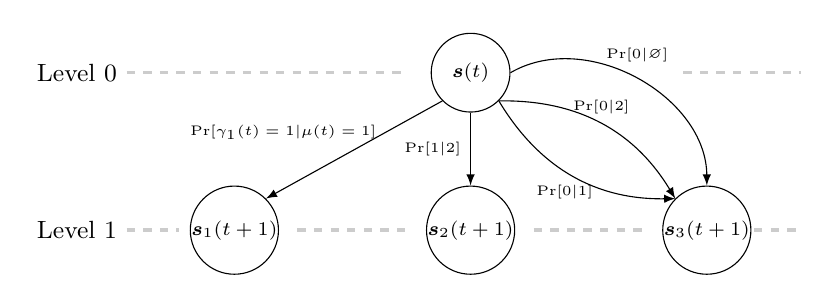
\begin{tikzpicture}[>=latex]
\def\nodesize{1cm}

%Root
\node (s0) at (0,0) [draw, circle, align=center, inner sep=0pt, minimum size=\nodesize] {\scriptsize$\boldsymbol{s}(t)$};

%Level 1
\node (s1) at (-3,-2) [draw, circle, align=center, inner sep=0pt, minimum size=\nodesize] {\scriptsize$\boldsymbol{s}_1(t+1)$};

\node (s2) at (0,-2) [draw, circle, align=center, inner sep=0pt, minimum size=1cm] {\scriptsize$\boldsymbol{s}_2(t+1)$};
\node (s3) at (3,-2) [draw, circle, align=center, inner sep=0pt, minimum size=1cm] {\scriptsize$\boldsymbol{s}_3(t+1)$};

\draw[->] (s0.south west) [] to node [above, pos=0.5, xshift=-.9cm] (aa) {\tiny$\text{Pr}{[\gamma_{1}(t)=1|\mu(t)=1]}$} (s1.north east);
\draw[->] (s0.south) [] to node [pos=0.5, left] (bb) {\tiny$\text{Pr}{[1|2]}$} (s2.north);
\draw[->, bend right] (s0.south east) [] to node [pos=0.5, below, xshift=-.1cm] (bb) {\tiny$\text{Pr}{[0|1]}$} (s3.north west);
\draw[->, bend left] (s0.south east) [] to node [pos=0.5, above, yshift=0cm] (cc) {\tiny$\text{Pr}{[0|2]}$} (s3.north west);
\draw[->, bend left=60] (s0.east) [] to node [pos=0.5, above, yshift=0.1cm] (cc) {\tiny$\text{Pr}{[0|\varnothing] }$} (s3.north);

\node (lev0) [] at (-5,0) {\small Level 0};
\draw [dashed,mygray, very thick] (lev0.east) to node [] (xyz) {} (-.8,0);
\draw [dashed,mygray, very thick] (2.7,0) to node [] (xyz) {} (4.2,0);

\node (lev1) [] at (-5,-2) {\small Level 1};

\draw [dashed, mygray,very thick] (lev1.east) to node [] (xyz) {} (-3.7,-2);
\draw [dashed,mygray,very thick] (-2.2,-2) to node [] (xyz) {} (-.8,-2);
\draw [dashed,mygray,very thick] (.8,-2) to node [] (xyz) {} (2.2,-2);
\draw [dashed,mygray,very thick] (3.6,-2) to node [] (xyz) {} (4.2,-2);


%%\draw[->] (sM.south) [out=-140,in=-40] to node [midway, below] (m2) {$p_1$} (s0.south);
%
%\draw[->, dashed] (s1.north east) -- (4.2,3);
%\draw[->, dashed] (s1.east) [] to node [] (bbb) {} (4.2,2.3);
%\draw[->, dashed] (s1.east) [] to node [pos=0.4, above] (bbbb) {} (4.2,1.7);
%\draw[->, dashed] (s1.south east) -- (4.2,1.2);
%
%\draw[->, dashed] (s2.north east) -- (4.2,0.6);
%\draw[->, dashed] (s2.east) [] to node [pos=0.4, above] (bbb) {} (4.2,0.2);
%\draw[->, dashed] (s2.east) [] to node [pos=0.4, above] (bbb) {} (4.2,-0.2);
%%\draw[->, bend right, dashed] (s2.east) [] to node [pos=0.4, above] (bbbb) {} (4.3,1.7);
%%\draw[->, dashed] (s2.south east) -- (4.2,1.2);
\end{tikzpicture}
} 
  \caption[FHS: Example tree structure with 2 sub-systems and finite horizon
  1]{Example $1$ level tree structure with $2$ sub-systems, i.e., $H=1$ and
  $N=2$. Each edge is labeled with the corresponding transition probability,
  i.e., $\Pr{[\gamma_{\mu(t)}(t)\mid \mu(t)]}$ as the conditional probability
  for the possible next network state to occur given the scheduling decision.
  The states $\textbf{s}_1$ and $\textbf{s}_2$ represent the cases where
  scheduled sub-systems successfully transmit their latest observation to the
  controller while $\textbf{s}_3$ represents the failure case where every
  sub-system fails to receive the transmitted packet.}
	\label{fig:FHStree}
\end{figure}

\section{Channel-aware Finite Horizon Scheduler} \label{sec:gescheduler}

We extend the introduced FHS with a \textit{Gilbert-Elliot channel-aware
Scheduler (GES)}, that takes channel state transitions for each link into
consideration. Similarly, GES utilizes the DP algorithm in order to solve the
$H$-stage problem. Namely, starting at state $\boldsymbol{s}(t)$ and time $t$,
the optimal final horizon cost $J^*(\boldsymbol{s}(t))$ is given by the last
step of the following algorithm:


\begin{center}
  \fbox{
    \parbox{0.9\textwidth}{
      Iterate backwards from $t'=t+H-1$ to $t'=t$
      \begin{equation} 
        \label{eq:dynamicprogramming}
        J_{t'}(\boldsymbol{s}(t')) = \min_{\mu(t') \in \mathcal{M}(\boldsymbol{s}(t'))} \E \left[ C(\boldsymbol{s}(t')) + J_{t' + 1}(\boldsymbol{s}(t' + 1))\right],
      \end{equation} 
      with the terminal cost: 
      \begin{equation}
        \label{eq:terminalcost}
        J_{t + H}(\boldsymbol{s}(t + H)) = C(\boldsymbol{s}(t + H)) 
      \end{equation}
      The expectation is taken with respect to the total MSE in the network as
      defined in Eq.~\eqref{eq:estimationerror} and Eq.~\eqref{eq:gfunction}.}
  }
\end{center}
  

According to the principle of optimality, if at each stage $t'$ the optimal
$\mu^*(t')$ action w.r.t to Eq.~\eqref{eq:dynamicprogramming} is taken, the
policy $\pi^* = \{\mu^*(t), \mu^*(t+1), \dots, \mu^*(t + H-1)\}$ is optimal and
achieves the minimum cost $J_{\pi^*}(\boldsymbol{s}(t)) = J_t(\boldsymbol{s}(t))
$. The proof can be found in \cite{bertsekas1995dynamic}.

\subsection{Algorithm}
The main difference to FHS lies in the size of the tree. The evolution of
network state $\boldsymbol{s}(t)$ with a GE channel not only depends on the
outcome of packet transmissions but is also simultaneously affected by the fact
that each link can change or retain their GE channel state $\boldsymbol{q}(t) $.
For instance, given $\delta_i(t)=1$, a successful transmission, i.e.,
$\gamma_i(t)=1$, can occur while Link $i$ changes or stays in Good/Bad state at
the same time. Provided any $\boldsymbol{s}(t')$, there exists $N$ individual
communication links. Thus, $2^N$ different GE channel transitions are possible
in the following time slot $t'+1$. Further, for each of these $2^N$ channel
states $\boldsymbol{q}(t'+1)$, $N+1$ network outcomes due to packet transmission
are possible, which correspond to $N$ successful transmissions for each link and
one common failed state. Compared to the FHS, each node in such a tree has $2^N$
times more child nodes. Fig.~(\ref{fig:GEStree}) shows a minimal tree for $N=2$,
$H=1$ and initial state $\boldsymbol{s}(t)=\left[t\quad t\quad a\quad b\quad
c\quad d\quad G\quad G \right]^T$.

In analogy to FHS, the backwards iteration employed by the DP algorithm can be
seen as traversing through all nodes of the tree level by level starting from
the leaf level while taking the optimal action at each level minimizing the
expected cost in the next level. Again, each node is assigned with a cost
obtained from Eq.~\eqref{eq:dynamicprogramming}. As a result, the operation of
the GE channel-aware FH scheduler can be summarized in the following steps:

\begin{enumerate}
	\item Initialize the current state $\boldsymbol{s}(t)$ as the root of a tree
	structure.
	\item Starting from the root, determine the possible actions at each node,
	i.e., $\mathcal{M}\boldsymbol{s}(t')$ for $\{t': t \leq t' < t + H \}$ and
	subsequently all possible next states $\boldsymbol{s}(t' + 1)$ when action
	$\mu(t')$ is taken.
	\item Add all possible next states as child nodes to the next level of the
	tree with the corresponding transition probabilities from the parent node.
	\item Repeat steps (2)-(4) until the $H$-th level of the tree is constructed.
	\item Assign costs to all states starting from the leaf nodes as in
	Eq.~\eqref{eq:dynamicprogramming} and \eqref{eq:terminalcost}.
\end{enumerate}

\begin{sidewaysfigure}
	\centering
  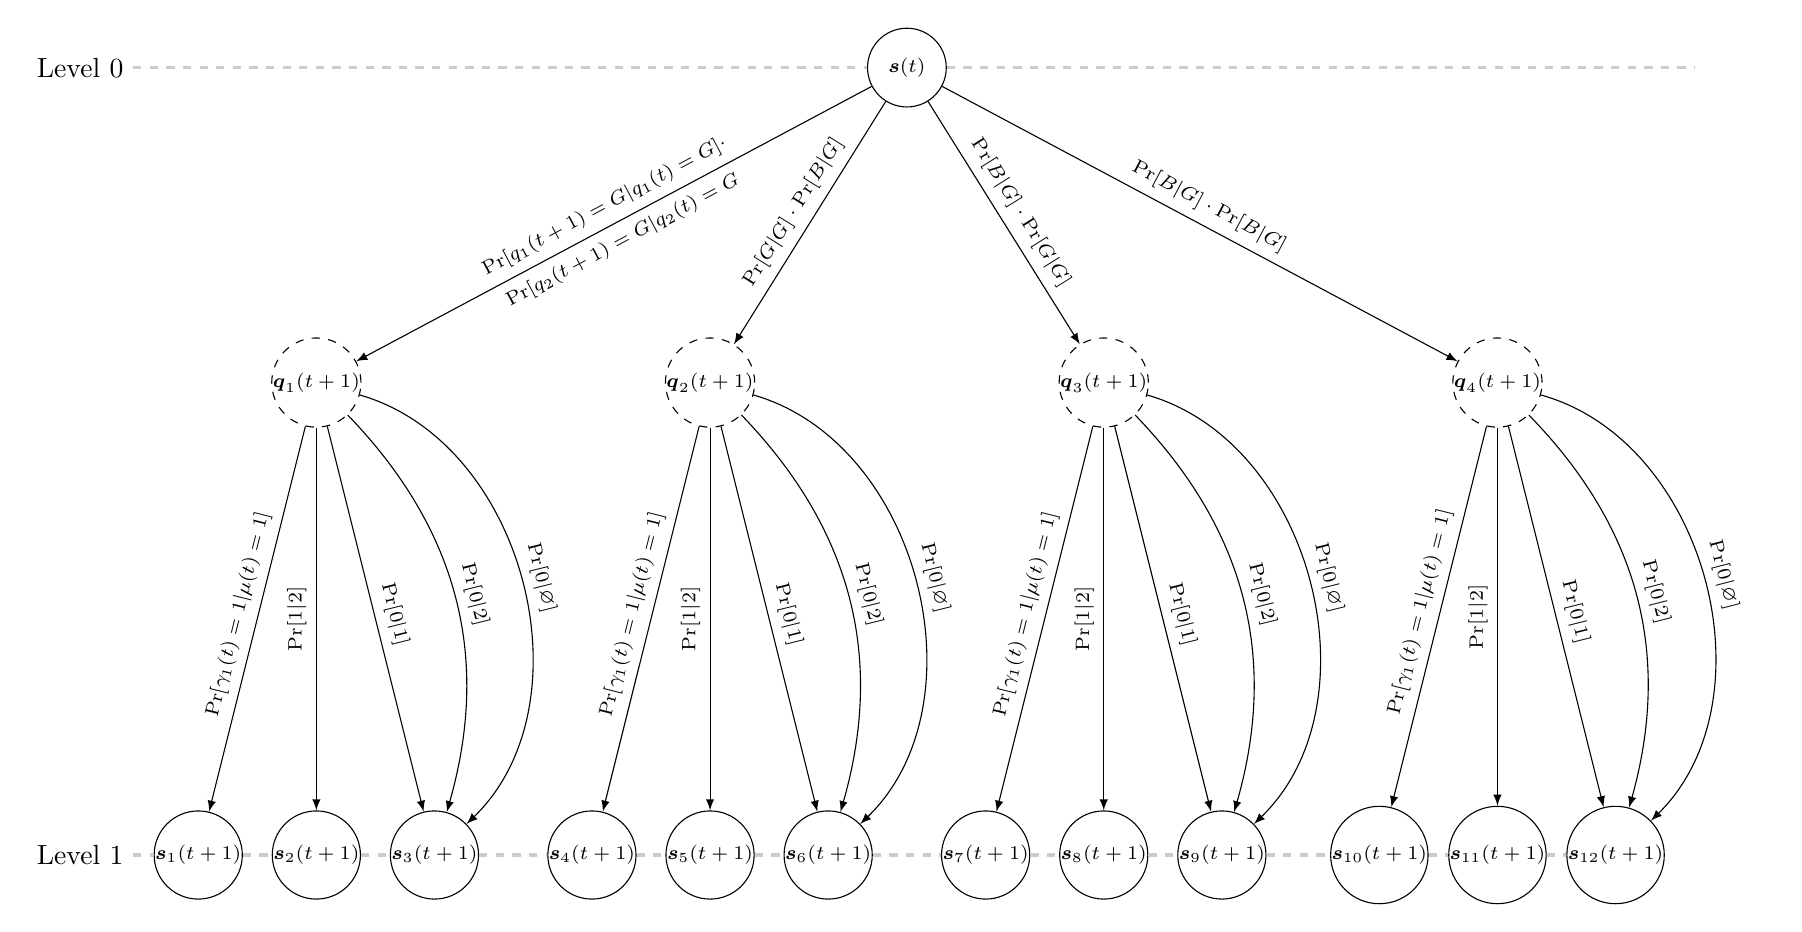
\begin{tikzpicture}[>=latex] 
\def\nodesize{1cm}
\def\leveliSize{-4cm}
\def\levelOneSize{-10cm}

%Root
\node (s0) at (0,0) [draw, circle, align=center, inner sep=0pt, minimum size=\nodesize] {\scriptsize$\boldsymbol{s}(t)$};

%Intermediate level
\node [dashed] (q1) at (-7.5,\leveliSize) [draw, circle, align=center, inner sep=0pt, minimum size=\nodesize] {\scriptsize$\boldsymbol{q}_1(t+1)$};
\node [dashed] (q2) at (-2.5,\leveliSize) [draw, circle, align=center, inner sep=0pt, minimum size=\nodesize] {\scriptsize$\boldsymbol{q}_2(t+1)$};
\node [dashed] (q3) at (2.5,\leveliSize) [draw, circle, align=center, inner sep=0pt, minimum size=\nodesize] {\scriptsize$\boldsymbol{q}_3(t+1)$};
\node [dashed] (q4) at (7.5,\leveliSize) [draw, circle, align=center, inner sep=0pt, minimum size=\nodesize] {\scriptsize$\boldsymbol{q}_4(t+1)$};

%Level 1
\node (s1) at (-9,\levelOneSize) [draw, circle, align=center, inner sep=0pt, minimum size=\nodesize] {\scriptsize$\boldsymbol{s}_1(t+1)$};
\node (s2) at (-7.5,\levelOneSize) [draw, circle, align=center, inner sep=0pt, minimum size=\nodesize] {\scriptsize$\boldsymbol{s}_2(t+1)$};
\node (s3) at (-6,\levelOneSize) [draw, circle, align=center, inner sep=0pt, minimum size=1cm] {\scriptsize$\boldsymbol{s}_3(t+1)$};
\node (s4) at (-4,\levelOneSize) [draw, circle, align=center, inner sep=0pt, minimum size=1cm] {\scriptsize$\boldsymbol{s}_4(t+1)$};
\node (s5) at (-2.5,\levelOneSize) [draw, circle, align=center, inner sep=0pt, minimum size=1cm] {\scriptsize$\boldsymbol{s}_5(t+1)$};
\node (s6) at (-1,\levelOneSize) [draw, circle, align=center, inner sep=0pt, minimum size=1cm] {\scriptsize$\boldsymbol{s}_6(t+1)$};
\node (s7) at (1,\levelOneSize) [draw, circle, align=center, inner sep=0pt, minimum size=1cm] {\scriptsize$\boldsymbol{s}_7(t+1)$};
\node (s8) at (2.5,\levelOneSize) [draw, circle, align=center, inner sep=0pt, minimum size=1cm] {\scriptsize$\boldsymbol{s}_8(t+1)$};
\node (s9) at (4,\levelOneSize) [draw, circle, align=center, inner sep=0pt, minimum size=1cm] {\scriptsize$\boldsymbol{s}_9(t+1)$};
\node (s10) at (6,\levelOneSize) [draw, circle, align=center, inner sep=0pt, minimum size=1cm] {\scriptsize$\boldsymbol{s}_{10}(t+1)$};
\node (s11) at (7.5,\levelOneSize) [draw, circle, align=center, inner sep=0pt, minimum size=1cm] {\scriptsize$\boldsymbol{s}_{11}(t+1)$};
\node (s12) at (9,\levelOneSize) [draw, circle, align=center, inner sep=0pt, minimum size=1cm] {\scriptsize$\boldsymbol{s}_{12}(t+1)$};

\draw[->] (s0) to node[sloped, above] {\scriptsize$\Pr[q_1(t+1)=G|q_1(t)=G]\cdot$} node[sloped, below] {\scriptsize$\Pr[q_2(t+1)=G| q_2(t)=G$} (q1);
\path[->] (s0) edge node [sloped, above] {\scriptsize$\Pr[G|G]\cdot \Pr[B|G]$} (q2);
\path[->] (s0) edge node [sloped, above] {\scriptsize$\Pr[B|G]\cdot \Pr[G|G]$} (q3);
\path[->] (s0) edge node [sloped, above] {\scriptsize$\Pr[B|G]\cdot \Pr[B|G]$} (q4);

\path[->] (q1) edge node [sloped, above] {\scriptsize$\Pr[\gamma_{1}(t)=1|\mu(t)=1]$} (s1);
\path[->] (q1) edge node [sloped, rotate=180, above] {\scriptsize$\Pr[1| 2]$} (s2);
\path[->] (q1) edge node [sloped, above]{\scriptsize$\Pr[0|1]$} (s3);
\path[->, bend left=30] (q1) edge node [sloped, above]{\scriptsize$\Pr[0|2]$} (s3);
\path[->, bend left=60] (q1) edge node [sloped, above]{\scriptsize$\Pr[0|\varnothing]$} (s3);

\path[->] (q2) edge node [sloped, above] {\scriptsize$\Pr[\gamma_{1}(t)=1|\mu(t)=1]$} (s4);
\path[->] (q2) edge node [sloped, rotate=180, above] {\scriptsize$\Pr[1| 2]$} (s5);
\path[->] (q2) edge node [sloped, above]{\scriptsize$\Pr[0|1]$} (s6);
\path[->, bend left=30] (q2) edge node [sloped, above]{\scriptsize$\Pr[0|2]$} (s6);
\path[->, bend left=60] (q2) edge node [sloped, above]{\scriptsize$\Pr[0|\varnothing]$} (s6);

\path[->] (q3) edge node [sloped, above] {\scriptsize$\Pr[\gamma_{1}(t)=1|\mu(t)=1]$} (s7);
\path[->] (q3) edge node [sloped, rotate=180, above] {\scriptsize$\Pr[1| 2]$} (s8);
\path[->] (q3) edge node [sloped, above]{\scriptsize$\Pr[0|1]$} (s9);
\path[->, bend left=30] (q3) edge node [sloped, above]{\scriptsize$\Pr[0|2]$} (s9);
\path[->, bend left=60] (q3) edge node [sloped, above]{\scriptsize$\Pr[0|\varnothing]$} (s9);

\path[->] (q4) edge node [sloped, above] {\scriptsize$\Pr[\gamma_{1}(t)=1|\mu(t)=1]$} (s10);
\path[->] (q4) edge node [sloped, rotate=180, above] {\scriptsize$\Pr[1| 2]$} (s11);
\path[->] (q4) edge node [sloped, above]{\scriptsize$\Pr[0|1]$} (s12);
\path[->, bend left=30] (q4) edge node [sloped, above]{\scriptsize$\Pr[0|2]$} (s12);
\path[->, bend left=60] (q4) edge node [sloped, above]{\scriptsize$\Pr[0|\varnothing]$} (s12);

\node (lev0) [] at (-10.5,0) {Level 0};
\draw [dashed,mygray, very thick] (lev0.east) to node [] (xyz) {} (s0.west);
\draw [dashed,mygray, very thick] (s0.east) to node [] (xyz) {} (10,0);

\node (lev1) [] at (-10.5,\levelOneSize) {Level 1};

\draw [dashed, mygray,very thick] (lev1.east) to node [] (xyz) {} (s1.west);
\draw [dashed, mygray,very thick] (s1.east) to node [] (xyz) {} (s2.west);
\draw [dashed, mygray,very thick] (s2.east) to node [] (xyz) {} (s3.west);
\draw [dashed, mygray,very thick] (s3.east) to node [] (xyz) {} (s4.west);
\draw [dashed, mygray,very thick] (s4.east) to node [] (xyz) {} (s5.west);
\draw [dashed, mygray,very thick] (s5.east) to node [] (xyz) {} (s6.west);
\draw [dashed, mygray,very thick] (s6.east) to node [] (xyz) {} (s7.west);
\draw [dashed, mygray,very thick] (s7.east) to node [] (xyz) {} (s8.west);
\draw [dashed, mygray,very thick] (s8.east) to node [] (xyz) {} (s9.west);
\draw [dashed, mygray,very thick] (s9.east) to node [] (xyz) {} (s10.west);
\draw [dashed, mygray,very thick] (s10.east) to node [] (xyz) {} (s11.west);
\draw [dashed, mygray,very thick] (s11.east) to node [] (xyz) {} (s12.west);

\end{tikzpicture}
 
  \caption[GES: Example tree structure with 2 sub-systems and finite horizon
  1]{Example $1$ level tree structure in a GE channel with $2$ sub-systems,
  i.e., $H=1$ and $N=2$. An initial state $\boldsymbol{s}(t)=\left[t\quad t\quad
  a\quad b\quad c\quad d\quad G\quad G \right]^T$ is assumed. $\boldsymbol{q}_
  {1\dots 4}$ resemble the $2^N=4$ possible GE channel states, each labeled with
  the corresponding transition probability, i.e., $\prod_{i=1}^{N}{\Pr[q_i(t+1)
  = G|q_i(t)=G]}$. Each of these intermediate nodes form the root of the tree
  shown in Fig.~(\ref{fig:FHStree}). In these $\Pr[\gamma_{\mu(t)}(t)\mid
  \mu(t)]$ stands for the conditional probability for the possible next network
  state to occur given the scheduling decision. For each $\boldsymbol{q}_{1\dots
  4}$, the first two child nodes correspond to the success state while the third
  child node is the shared failed state.}
	\label{fig:GEStree}
\end{sidewaysfigure}

Furthermore, it should be emphasized, that although the obtained optimal policy
$\pi^*$ consists of $H$ optimal scheduling decisions, only the action at level 0
is applied. This is because the root of the tree changes after each slot,
causing the remaining $H-1$ actions to be not optimal anymore. Hence, steps
(1)-(6) have to be repeated every time slot as well. 

\subsection{Complexity}

The complexity of the GES is governed by both the construction of the tree and
the search for the shortest path. The worst-case scenario in terms of complexity
takes place when all sub-systems in the network are sampled every slot, i.e.,
$D_i=1$. Then every node in the tree will have $2^N(N+1)$ child nodes. The total
amount of nodes $n$ in a perfect $m$-ary tree is computed by:

\begin{equation}
  n = \sum_{i=0}^{h}m^i = \frac{m^{h+1}-1}{m-1}
\end{equation}
Applied to our tree with $m=2^N(N+1)$ and $h=H$: 
\begin{equation}
  n = \frac{(2^N(N+1))^{H+1}-1}{2^N(N+1)-1} 
\end{equation} 

Depending on how often each node is visited in the concrete implementation, the
complexity becomes $c \cdot n$, where $c$ is a positive constant. However, in
simplified Big-O notation, $c$ can be omitted and the complexity is given as
$\mathcal{O}(2^N\cdot N^H)$. This corresponds to a brute-force search for the shortest
path in our constructed tree. The amount of nodes and complexity can be reduced
by increasing the sampling period. As packets are only generated at sampling
events, if a sub-systems succeeds to transmit its plant measurement from that
sampling period, it will not have any new packet to transmit for the rest of
sampling period. Thus, the number of possible actions at these states will not
incorporate said sub-systems. In other words, if $t_{i,g}(t) = t_{i,r}(t)$, then
$i \not \in \mathcal{M}(t)$, thereby, reducing the amount of nodes in the next
level.

\chapter{Evaluation} \label{ch:evaluation}

In this chapter, we implement FHS and GES into a centralized wireless resource
scheduling problem with underlying GE channel and evaluate the behavior as well
as the performance of our proposed method in simulations. To provide an
appropriate comparison, in Sec.~\ref{sec:setup} we describe our choices for the
simulation environment and introduce three testing scenarios with different
network configurations. Finally, we present and discuss the results of different
simulations in Sec.~\ref{sec:results}. 

\section{Simulation Setup} \label{sec:setup}
% Details regarding implementation and/or simulation are given in this chapter.
% The considered setup and the parameters used are introduced and discussed. Also,
% the general evaluation methods can be presented. (Note: Code should not be part
% of this chapter. If it makes sense to introduce it into the thesis, it should be
% placed in the appendix.)

Suppose a minimal simulation environment comprising of $N=3$ control sub-systems
sharing a GE wireless channel to demonstrate the benefit of finite horizon
minimization. In order to provide intuitive and illustrative results, we
consider scalar sub-systems in the evaluation. Each sub-system is chosen to have
different plant system dynamics, with increasing unstable system matrices, i.e.,
$A_{1,2,3} = \left\{1.0, 1.25, 1.5\right\}$. The input matrix is given by $B_i =
1.0, \forall i$. The control sub-systems are initialized with $x_i[0] = w_i[0]$
for all $i$ and system noise is characterized by $w_i[k]\sim \mathcal{N}(0,1)$,
i.e., $\Sigma_i=1$. Among the simulated sub-systems, $A_3=1.5$ represents the
most challenging application, as its system state evolves the most within a
control time step $k$. Moreover, sub-systems are sampled periodically every 3
slots, i.e., $D_i=3$. To enable non-synchronized sampling, we determine the
initial sampling event randomly from a discrete uniform distribution as $t_{i,o}
= \mathcal{U}\{0, D_i-1\}$. The feedback gain matrix is given by
$\boldsymbol{L}^*_i = A_i$, which corresponds to deadbeat control strategy. 

\begin{table}[htb]
  \begin{center}
  \begin{tabular}{|lc|c|c|c|} 
  \hline
  \multicolumn{2}{|c|}{\textbf{Channel model parameters}} & \textbf{Scenario 1} & \textbf{Scenario 2} & \textbf{Scenario 3} \\
  \hline \hline
  Loss in Good & $p_G$ & 0.25 & 0.25 & 0.0011 \\ 
  Loss in Bad & $p_B$ & 0.75 & 0.75 &  0.7734 \\ 
  Failure rate & $f$ & 0.3 & 0.1 & 0.0024 \\ 
  Recovery rate & $r$ & 0.3 & 0.1 & 0.0832 \\
  \hline
  Stationary probability Bad & $\pi_G$ & 0.5 & 0.5 & 0.972 \\
  Stationary probability Good & $\pi_B$ & 0.5 & 0.5 & 0.028 \\
  Average error probability & $p_E$ & 0.5 & 0.5 & 0.0227 \\
  Mean sojourn time in Good & $T_G$ & 3.33 & 10 & 416.66 \\
  Mean sojourn time in Bad & $T_B$ & 3.33 & 10 & 12 \\
  \hline
  \end{tabular}
  \end{center}
  \caption{Summary of evaluation scenarios and their Gilbert-Elliot channel parametrization}
  \label{tab:scenarios}
\end{table}

Table~\ref{tab:scenarios} depicts the 3 chosen scenarios and their respective GE
channel parametrization. Scenario 1 and 2 resemble challenging GE channels,
where on average half of the packets transmitted are lost. Further, due to
symmetrical state transition probabilities, the channel will be in good and bad
states 50\% of the simulation time on average each. $f$ and $r$ merely differ in
absolute values, making the second channel prone to longer burst errors. To
evaluate scheduler performance in a real-life scenario, we have adopted the GE
parameters for scenario 3 from experiments conducted in
\cite{frohn2011analyzing}. Here, measurements are obtained from an indoor
wireless testbed based on the IEEE 802.11n standard. Obtained network trace is
then used to find analytical GE parameters using the \textit{Baum-Welch
algorithm} \cite{baum1970maximization}. Compared to the first two settings,
scenario 3 provides a good channel with significantly lower average loss
probabilities and stays in the good state for the majority of time. For each
scenario we vary the finite Horizon $H=\left\{ 1, \cdots, 10\right\}$ for FHS
and $H=\left\{ 1, \cdots, 4\right\}$ for GES to study its effect on AoI and MSE.
Each configuration is simulated for a duration of $D=20000$ time slots and
repeated $R=200$ times. 

\subsection{Performance Metrics} 

We evaluate scheduling performance in terms of the following metrics. In every
simulation, the average mean squared error of a sub-system $i$ at each slot is
measured as:

\begin{equation*}
  MSE_i = \dfrac{1}{D} \sum_{t=1}^{D}{(\boldsymbol{e}_i(t))^T \boldsymbol{e}_i(t)},
\end{equation*}

where $\boldsymbol{e}_i(t)$ is the estimation error defined in
Eq.~\eqref{eq:estimationerror}. In addition, we analyze the average MSE in the
network given by:

\begin{equation*}
  \overline{MSE} = \dfrac{1}{N} \sum_{i=1}^{N}{MSE_i}
\end{equation*}

MSE indicates the deviation of the estimated state from its true state, thus
quantifying estimation accuracy of estimator $\estimator$ as well as the
uncertainty in the controlled process. In the same fashion, we measure
information staleness at $\estimator$ by means of individual and total average
AoI as follows:

\begin{align*}
  \Delta_i &= \dfrac{1}{D} \sum_{t=1}^{D}{\Delta_i(t)}, \\
  \overline{\Delta} &= \dfrac{1}{N} \sum_{i=1}^{N}{\Delta_i}
\end{align*}

\section{Results and Discussion} \label{sec:results}
% Results of the performed investigations are presented here. Interpretations for
% the observed effects are given and the impact of investigations is discussed. 

\subsection{Age-of-Information Performance}

\begin{figure}[htb]
  \centering
  \begin{subfigure}{0.49\textwidth}
    \centering
    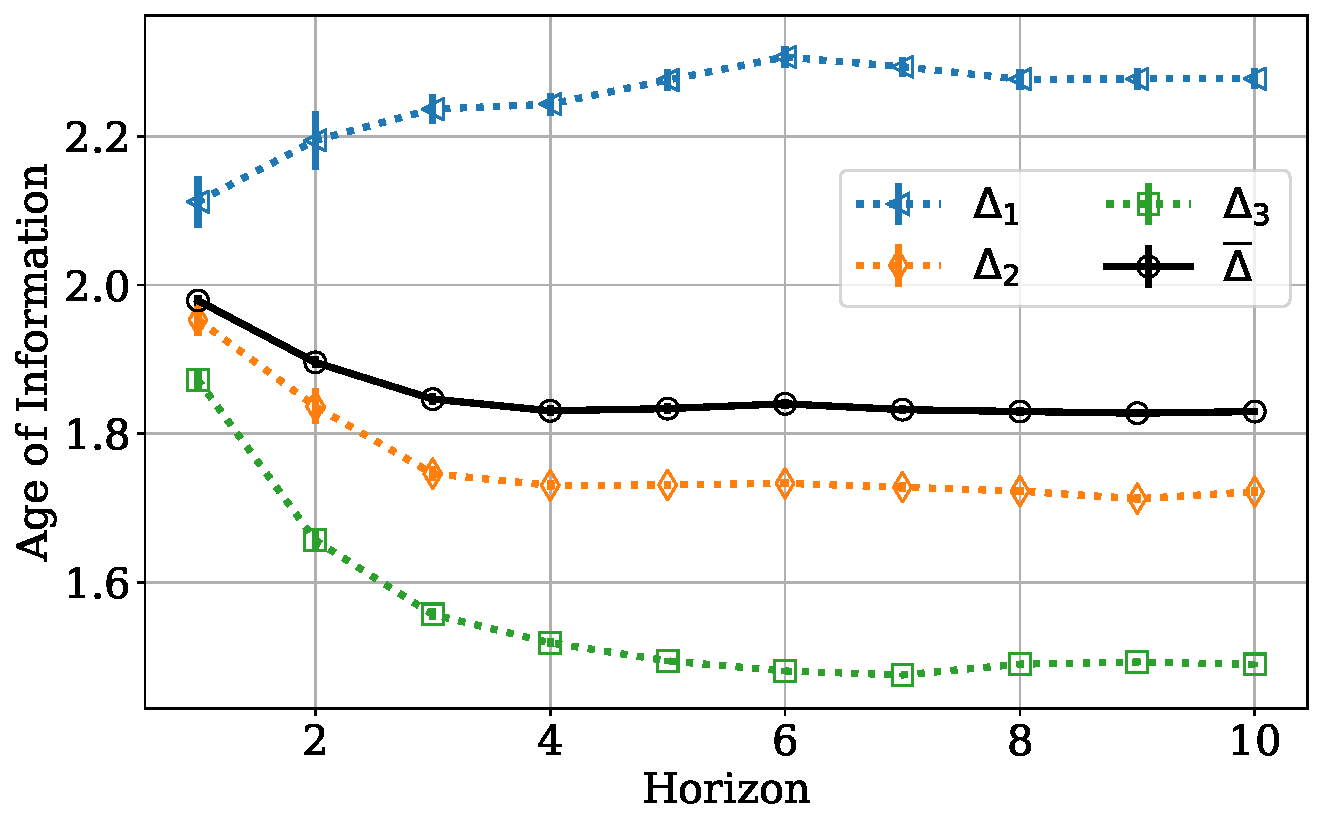
\includegraphics[width=\textwidth]{FHS1_AoI_against_H_separate}
    \caption{Scenario 1 with FHS}
  \end{subfigure}
  \hfill
  \begin{subfigure}{0.49\textwidth}
    \centering
    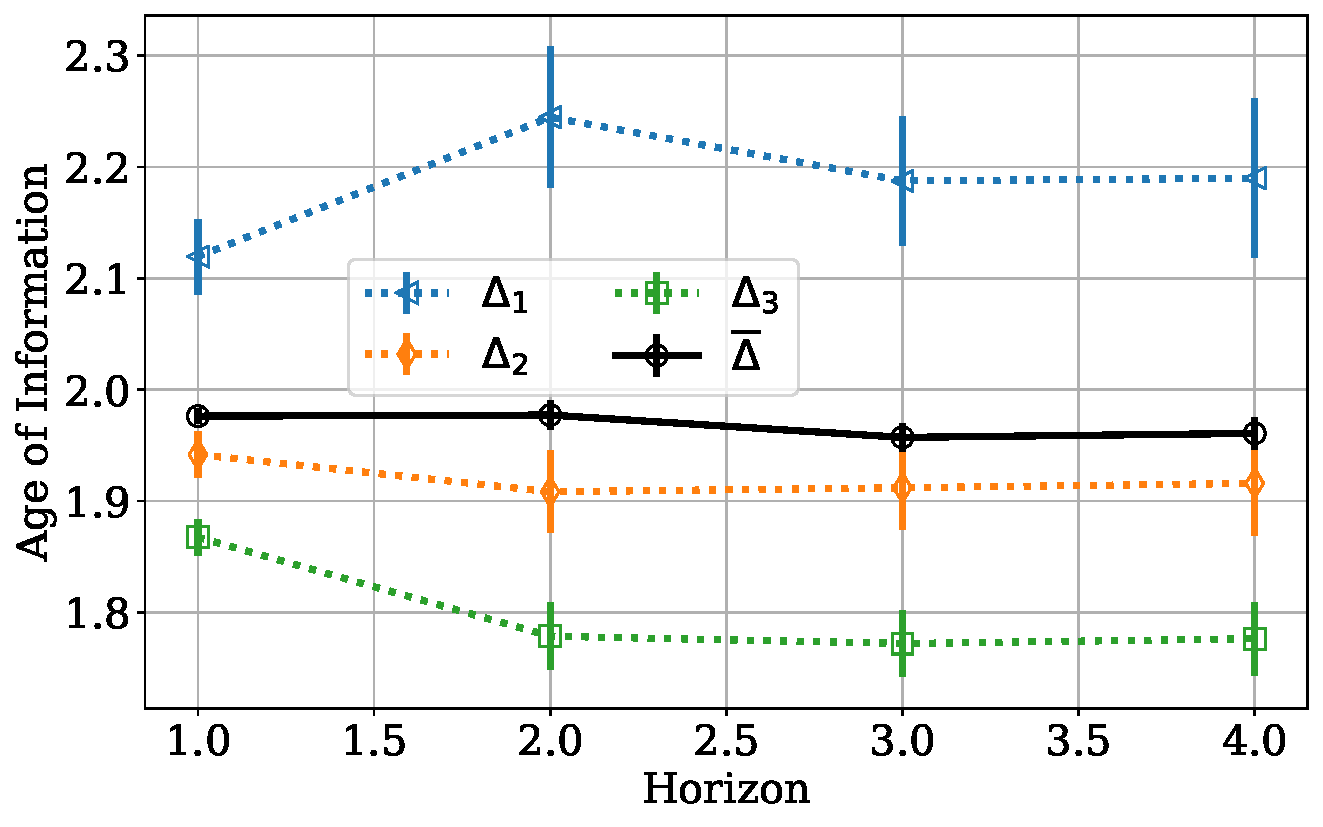
\includegraphics[width=\textwidth]{GES1_AoI_against_H_separate}
    \caption{Scenario 1 with GES}
  \end{subfigure}
\caption[Scenario 1: Average AoI vs. finite horizon $H$]{Achieved average AoI
vs. finite horizon $H$ for FHS and GES. Solid lines $\overline{\Delta}$
illustrate the average AoI in the network per time slot. Dashed lines
$\Delta_1$, $\Delta_2$ and $\Delta_3$ show the average AoI per time slot of each
class with $A_1 = 1.0$, $A_2=1.25$ and $A_3=1.5$, respectively. Vertical bars
represent $95\%$ confidence intervals for $R=200$ simulation runs.}
\label{fig:AoIseperate}
\end{figure}

Fig.~\ref{fig:AoIseperate} depicts the resulting AoI performance among
sub-systems sharing the network for scenario 1. We observe that the average AoI
differs for each sub-system. This is an expected result, since FHS and GES aim
to minimize the short-term MSE trajectory, regardless on how often a loop is
granted medium access. This behavior can be elaborated with the help of
Fig.~\ref{fig:networkshare} which illustrates average network shares of
individual sub-systems. It directly reflects the scheduling decisions taken by
our proposed algorithm. We can examine that the scheduler grants more medium
access to sub-systems, which are expected to produce higher costs. In
particular, we can see that the most critical sub-system $A_3 = 1.5$ is
scheduled in average more frequently. This leads to unequal distribution of
network resource, prioritizing control application the scheduler deems for more
expensive in terms of cost. We further observe that average AoI is inversely
proportional to network share. This make sense since in our scenario, a lower
AoI indicates a more frequent update rate. 

\begin{figure}[p]
\centering
\begin{subfigure}{0.49\textwidth}
  \centering
  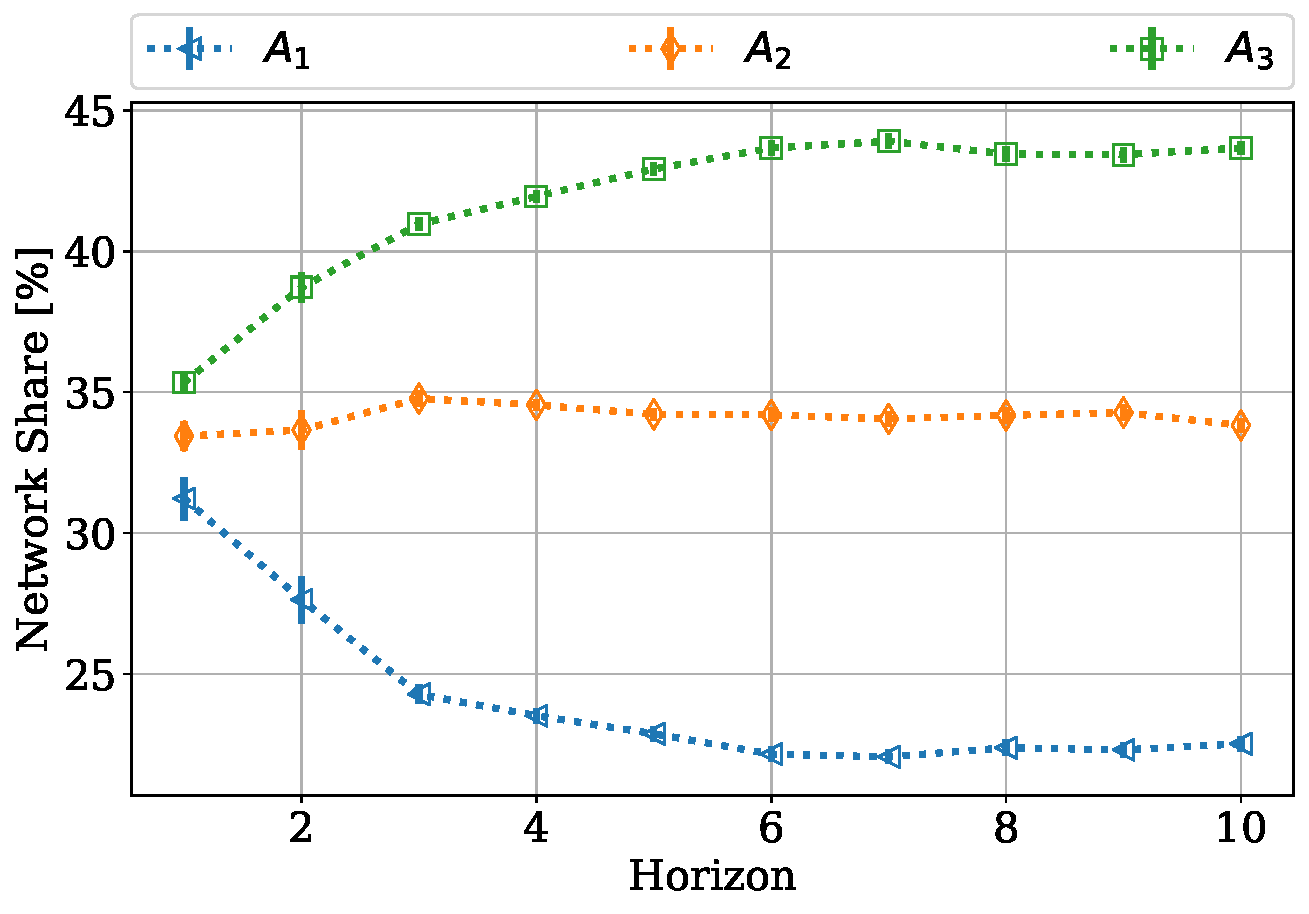
\includegraphics[width=\textwidth]{FHS1_NS_against_H_separate}
  \caption{Scenario 1 with FHS}
\end{subfigure}
\hfill
\begin{subfigure}{0.49\textwidth}
  \centering
  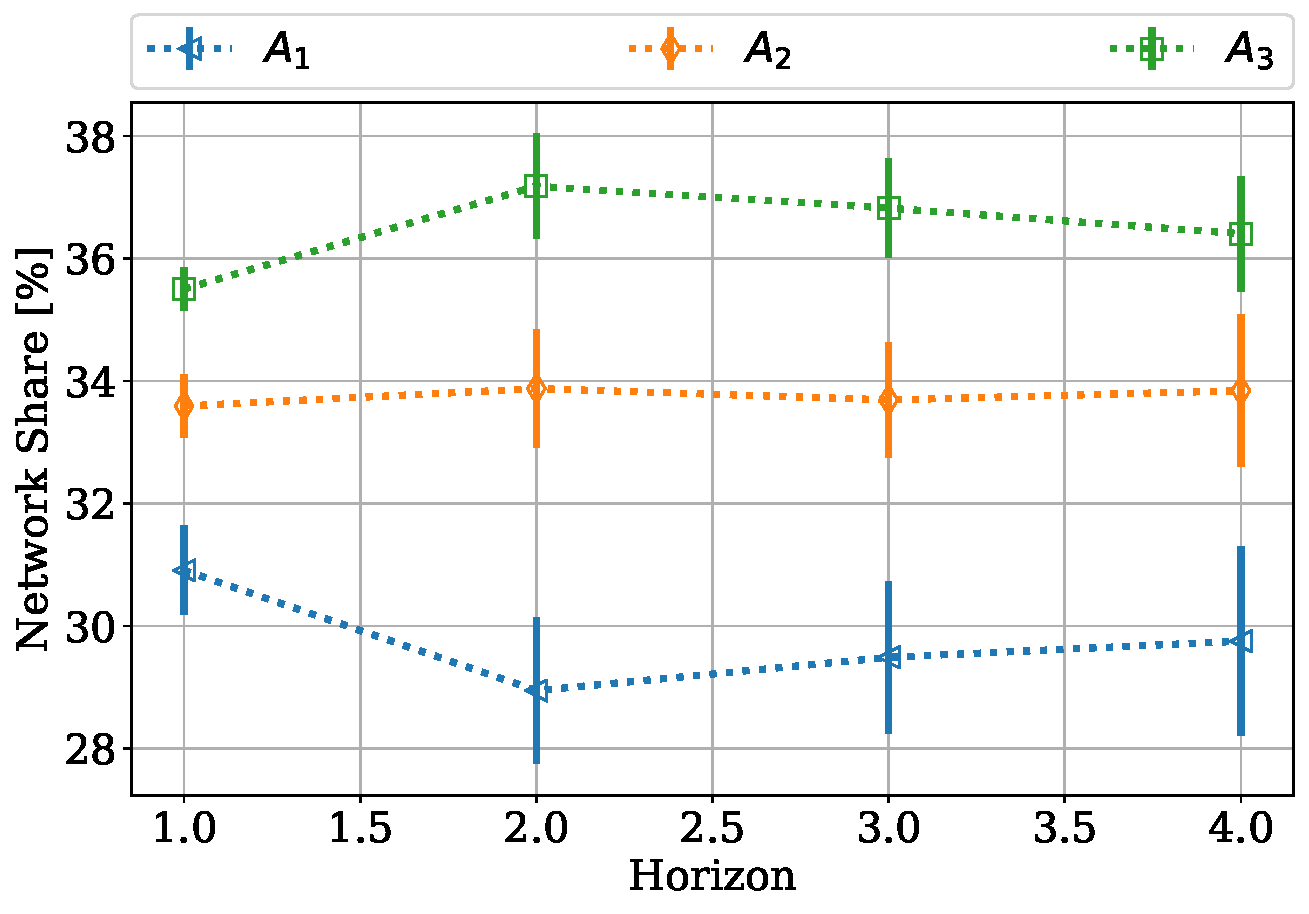
\includegraphics[width=\textwidth]{GES1_NS_against_H_separate}
  \caption{Scenario 1 with GES}
\end{subfigure}
  \caption[Scenario 1: Network share among heterogenous subsystems vs. finite
  horizon $H$]{Network share among simulated sub-systems vs. finite horizon $H$
  over $R=200$ simulation runs. Out of three control loops, only one sub-system
  is allowed to transmit simultaneously. A network share $\alpha_i\%$ indicates
  that the $i$-th sub-system was granted channel access $\alpha_i\%$ of the time
  in average.} 
  \label{fig:networkshare}
\end{figure}

\begin{figure}[p]
  \centering
  \begin{subfigure}{0.49\textwidth}
    \centering
    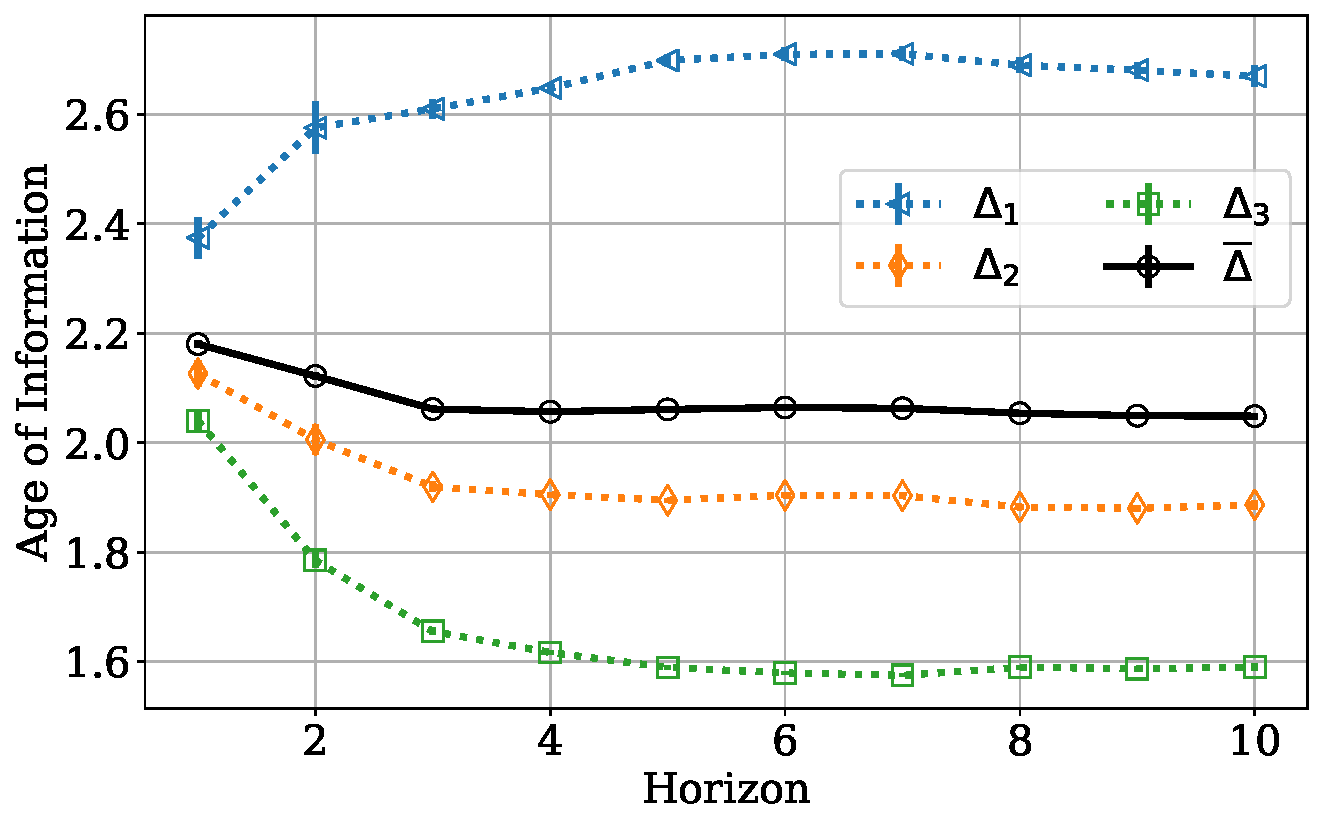
\includegraphics[width=\textwidth]{FHS2_AoI_against_H_separate}
    \caption{Scenario 2 with FHS}
  \end{subfigure}
  \hfill
  \begin{subfigure}{0.49\textwidth}
    \centering
    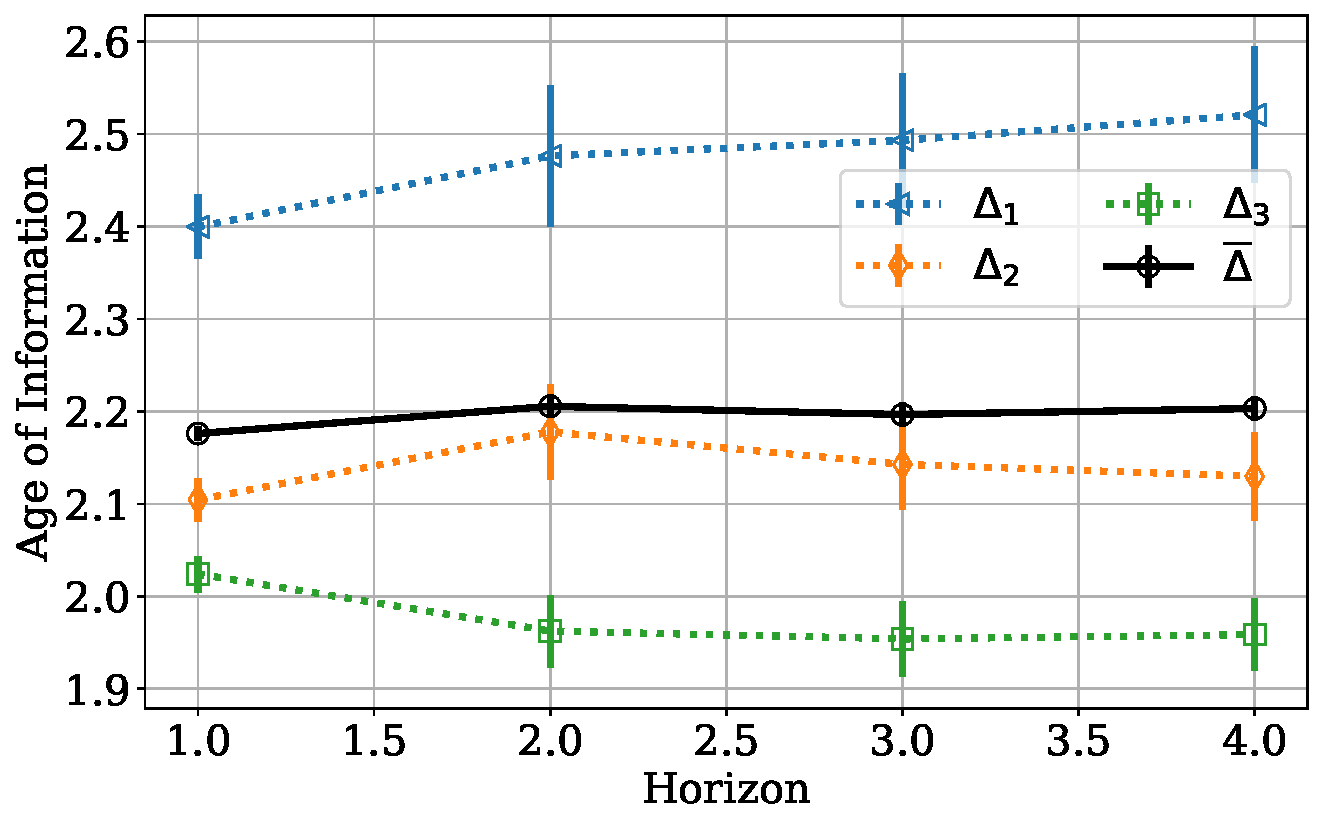
\includegraphics[width=\textwidth]{GES2_AoI_against_H_separate}
    \caption{Scenario 2 with GES}
  \end{subfigure}
  \begin{subfigure}{0.49\textwidth}
    \centering
    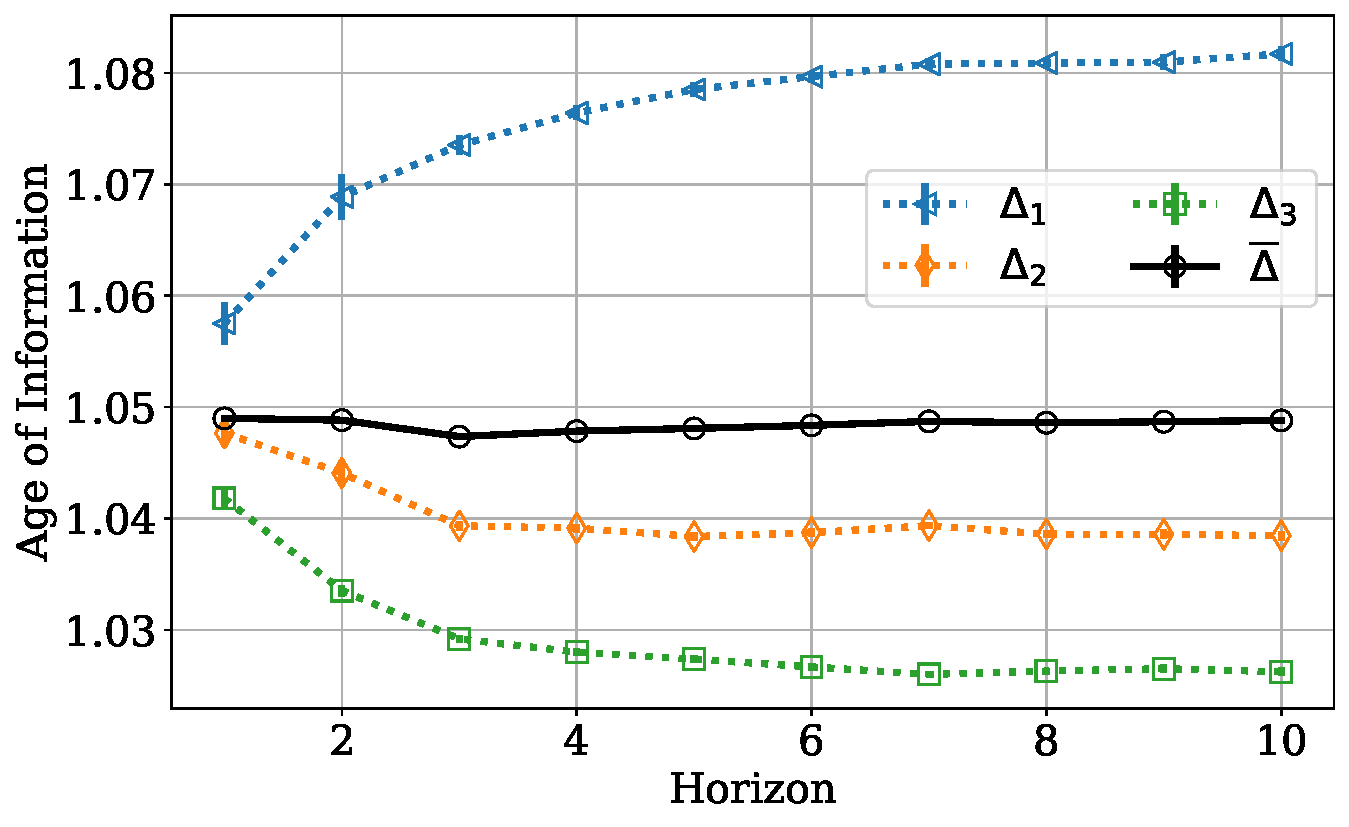
\includegraphics[width=\textwidth]{FHS3_AoI_against_H_separate}
    \caption{Scenario 3 with FHS}
  \end{subfigure}
  \hfill
  \begin{subfigure}{0.49\textwidth}
    \centering
    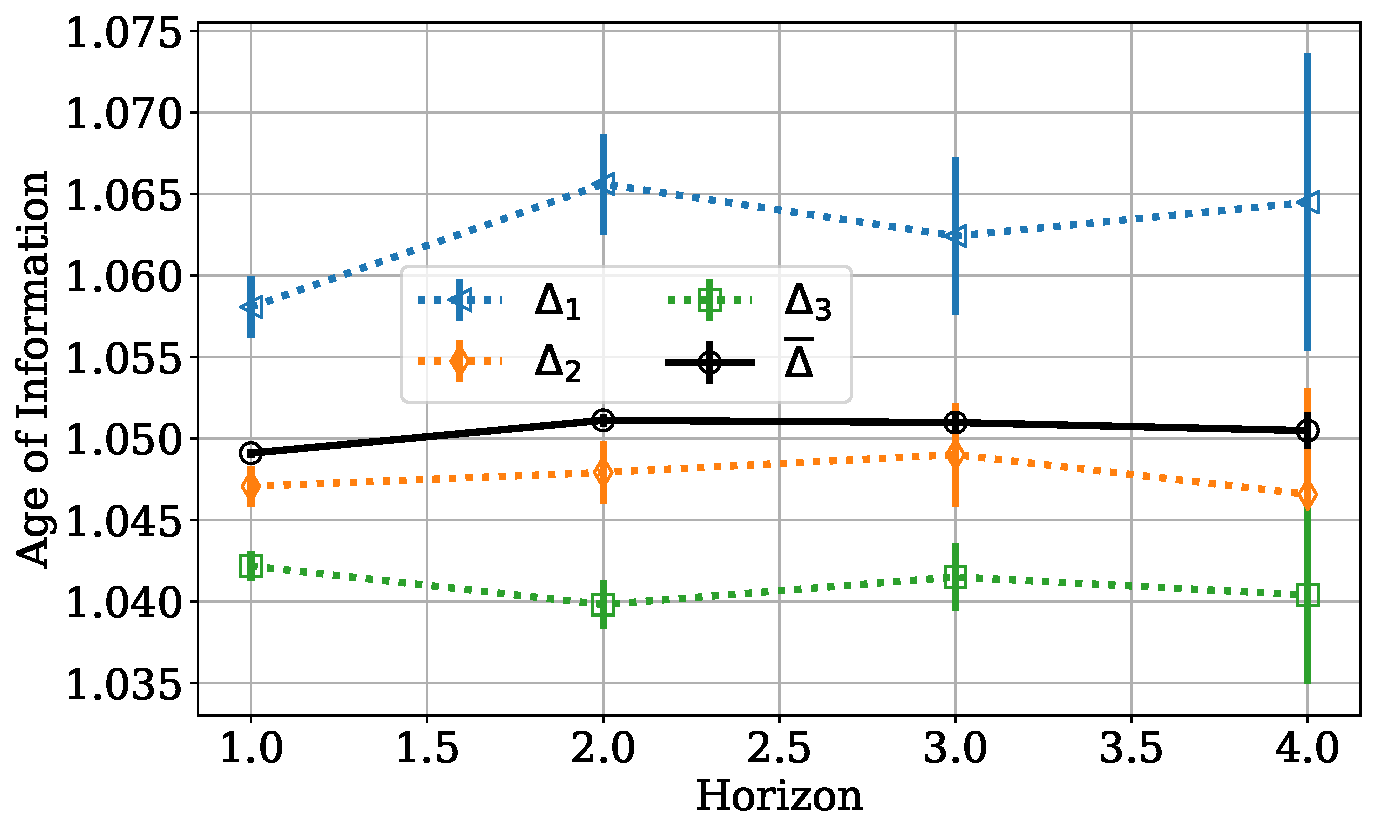
\includegraphics[width=\textwidth]{GES3_AoI_against_H_separate}
    \caption{Scenario 3 with GES}
  \end{subfigure}
  \caption{Scenario 2 \& 3: Average AoI vs. finite horizon $H$}
  \label{fig:AoIseperate2}
\end{figure}

In addition, for FHS we observe a falling trend in $\Delta_2$ and $\Delta_3$ as
$H$ increases. This effect results from the increasing foresight of the
scheduler for possible high future costs in case of consecutive unsuccessful
transmissions. In contrast, GES seems to equalize resource distribution among
sub-systems starting from $H=3$. We interpret this as a result of GES
considering possible GE channel state transitions, while FHS simply assumes the
links to be constant for the next $H$ time slots. For instance, the high cost of
not updating sub-system $A_3=1.5$ is compensated through a high probability of
its link transiting to good state.

Fig.~\ref{fig:AoIseperate2} plots AoI performance for scenario 2 and 3,
respectively. For FHS the same characteristic trend for AoI can be observed.
However, absolute AoI values are shifted upwards for scenario 2 and downwards
for scenario 3. This is a result of different channel qualities in each
scenario. Although the average packet loss probability is equal for scenario 1
and 2, the second channel is expected to stay longer in bad state. This results
in longer consecutive packet losses, thus increasing AoI in the network. The
effect on scenario 3 can be explained analogously.

\subsection{Age-of-Information Distribution}

\begin{figure}[htb]
  \centering
  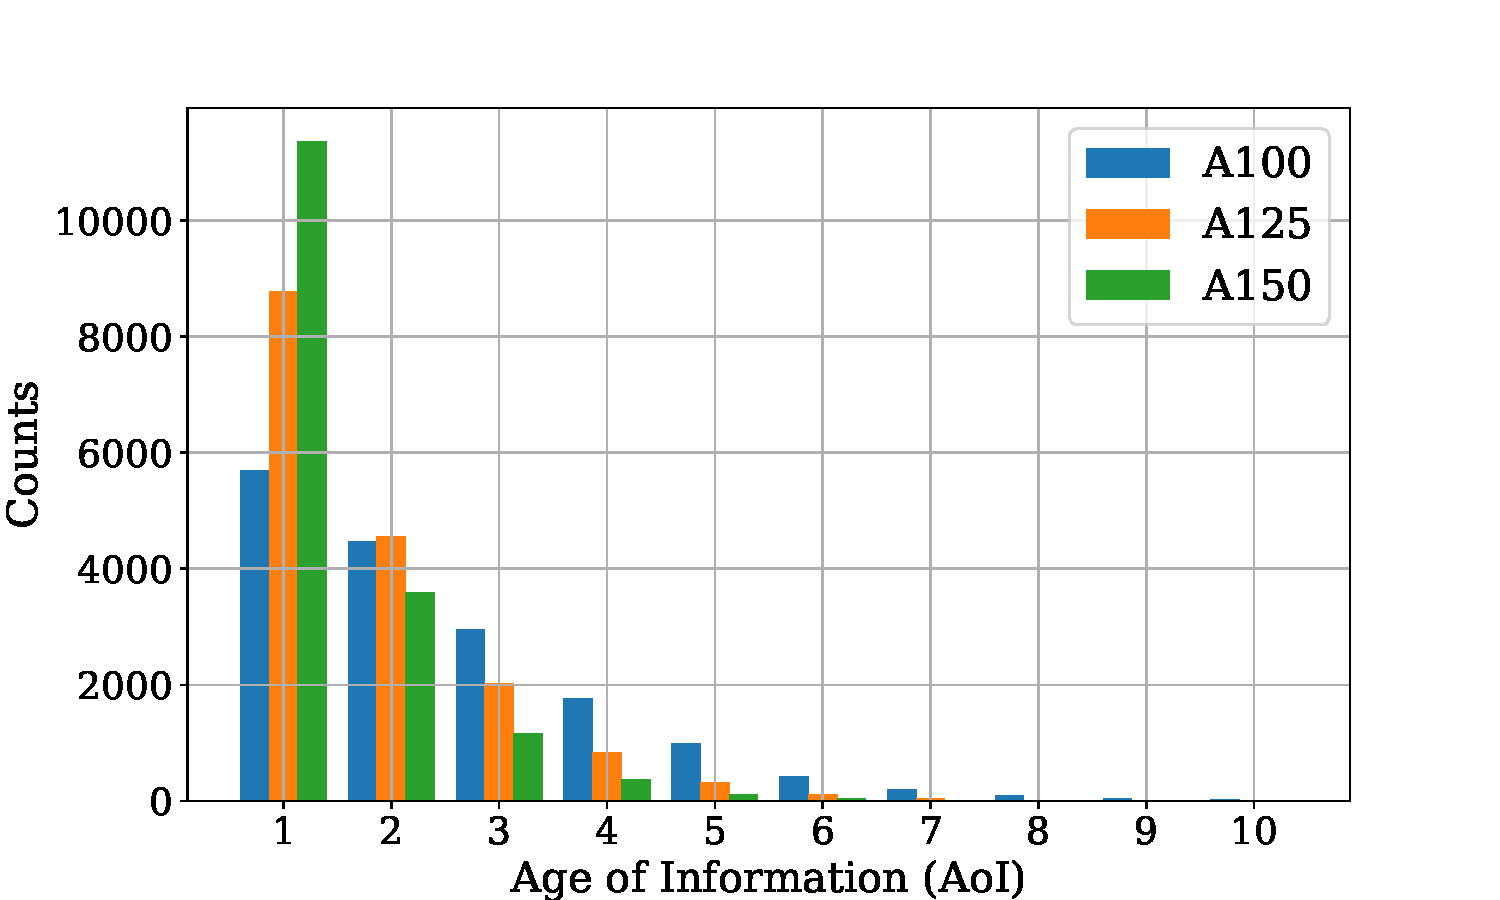
\includegraphics[width=0.6\textwidth]{AoI_Histogram_N3}
  \caption[Scenario 1: Measurement of AoI distribution]{Histogram of perceived
  AoI at controller $\controller$ for simulated sub-systems $A_i=\left\{1.0,
  1.25, 1.5\right\}$ with channel parameters according to Scenario 1. Network
  resources are managed by FHS with $H=2$.} 
  \label{fig:AoIHist}
\end{figure}

Merely examining expected AoI might be misleading and not sufficient when it
comes to time-critical-requirements of underlying sub-systems
\cite{ayan2020probability}. To have a deeper insight of age dependent
performance, we have exemplary measured AoI distribution in the network for one
simulation run consisting of $R=50000$ time slots in scenario 1.
Fig.~\ref{fig:AoIHist} shows the amount of time slots each sub-system were in
the state of respective AoI for FHS with $H=2$. As expected, the most up-to-date
plant measurements were available to task-critical sub-systems. This is seen in
$A_3$ having the highest 1 count, followed by $A_2$ and $A_1$. We can see the
consequence of the scheduler distributing network resources unequally, in a
shift of counts for higher AoI values, where $A_1$ has the highest counts and
$A_1$ the lowest.
  
\cite{ayan2020probability} provides a closed-form expression for the AoI
probability mass function in single and multi-hop networks. In contrast, they
consider a single NCS transmitting over a multi-hop network with time-invariant
packet loss probabilities. Although not directly applicable, we observe a
similar geometric AoI distribution in our measurement. Fig.~\ref{adx:aoiHist}
includes the AoI histogram for the equivalent scenario studied in the paper and
validates their analytical probability mass function for single hop networks.

\subsection{Remote Estimation Performance}

\begin{figure}[htb]
  \centering
  \begin{subfigure}{0.49\textwidth}
    \centering
    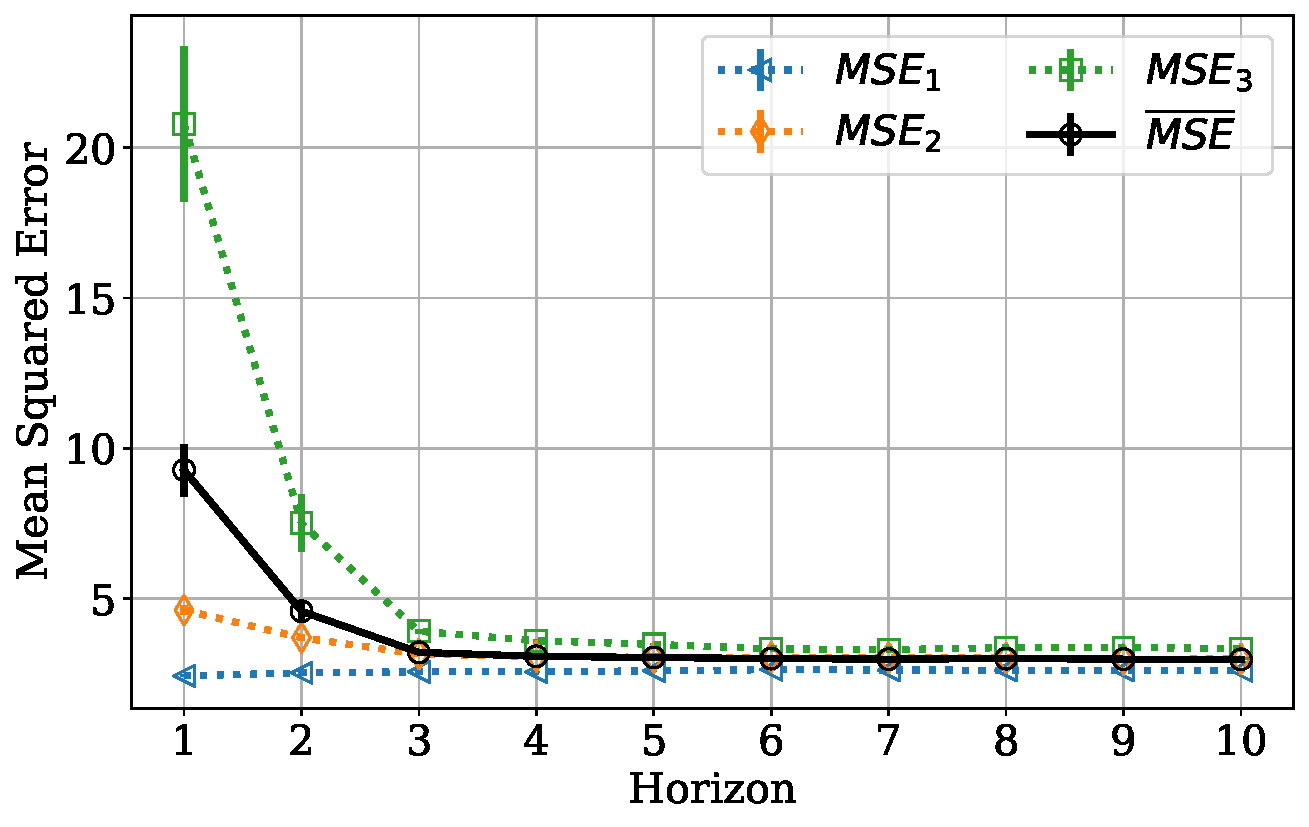
\includegraphics[width=\textwidth]{FHS1_MSE_against_H_separate}
    \caption{Scenario 1 with FHS}
    \label{fig:surprise}
  \end{subfigure}
  \hfill
  \begin{subfigure}{0.5\textwidth}
    \centering
    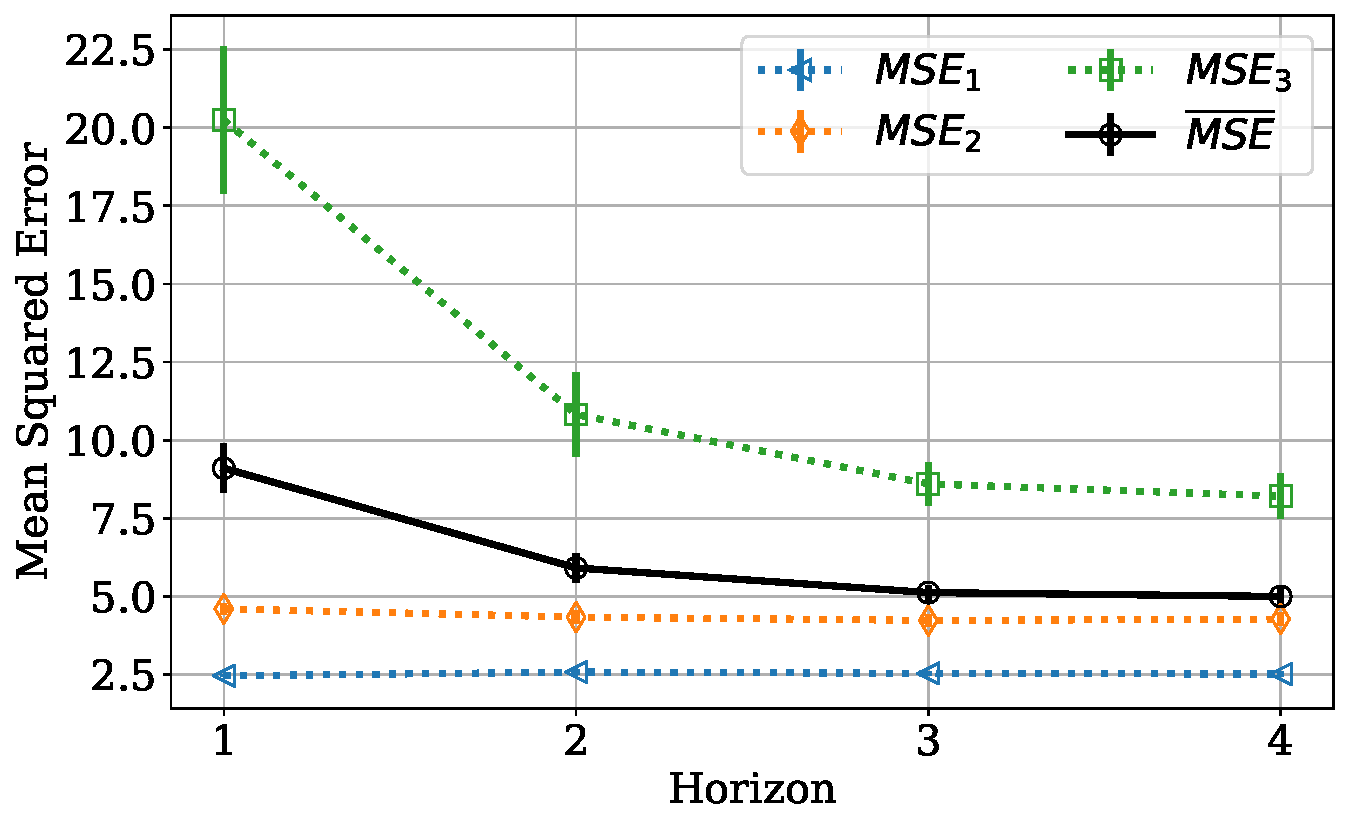
\includegraphics[width=\textwidth]{GES1_MSE_against_H_separate}
    \caption{Scenario 1 with GES}
  \end{subfigure}
  \caption[Scenario 1: Average MSE vs. finite horizon $H$]{Achieved average
  MSE vs. finite horizon $H$ for FHS and GES. Solid lines $\overline{MSE}$
  illustrate the average MSE in the network per time slot. Dashed lines
  $MSE_1$, $MSE_2$ and $MSE_3$ show the average MSE per time slot of each
  class with $A_1=1.0$, $A_2=1.25$ and $A_3=1.5$, respectively. Vertical bars
  represent $95\%$ confidence intervals for $R=200$ simulation runs.}
  \label{fig:MSEavg}
\end{figure}

Putting all our insights of the previous subsections together, we next focus on
our main performance metric $MSE_i$. Fig.~\ref{fig:MSEavg} depicts the
estimation performance achieved by FHS and GES in scenario 1 for varying $H$.
For both FHS and GES, a significant reduction of $\overline{MSE}$ can be seen as
we increase the horizon from $H=1$ to $H=2$. However, beyond $H=2$, as the
scheduler gets more farsighted, the performance gain diminishes and the MSE
trajectory converges. We further examine our scheduler's long-term behavior. As
$H$ increases, the $MSE_i$ lines tend to meet. This effect result from equal
weighing of individual sub-system MSE when obtaining the network cost defined in
Eq.~\eqref{eq:gfunction}. This in turn leads to equal long-term averages as the
scheduling decisions become more ``long-term optimal''. Moreover, notice how
sub-system 3 is the one with the highest MSE in the network, although $\Delta_3$
is the lowest among all $\Delta_i$. This is because according to
Eq.~\eqref{eq:estimationerror} estimation error is obtained through AoI and the
underlying system dynamics, meaning that estimation errors propagate differently
for every sub-system.

To our surprise, comparing absolute values of $\overline{MSE}$ between FHS and
GES, suggests that GES does not improve estimation accuracy compared to its base
scheduler in a GE-channel although it is aware of possible channel transitions.
Furthermore, we hoped to observe a slight increase of average MSE in
Fig.~\ref{fig:surprise}. In a channel with mean sojourn time of 3.33, we
initially expected to observe an increase starting from $H=4$ as the scheduler
plans too many time slots ahead, which would result in possible bad schedules
taken in terms of estimation performance.

Fig.~\ref{fig:MSEavg2} plots FHS and GES estimation performance for scenario 2
and 3. We examine a shift for MSE trajectories with FHS for both scenarios as
already seen with AoI, which can also be explained with changing channel
qualities. However, in the case of GES in scenario 2, estimation error of
subs-system 3 increases after $H=3$. We interpret this effect as the result of
the channel being too random, which the scheduler can not react to as it merely
considers estimation errors in expectation. Thus, in combination with the longer
burst errors, the bad scheduling decisions propagate into growing estimation
errors. As scenario 3 has the best channel quality on average, an overall
decreasing trend is observed for GES.

\begin{figure}[htb]
  \centering
  \begin{subfigure}[b]{0.49\textwidth}
    \centering
    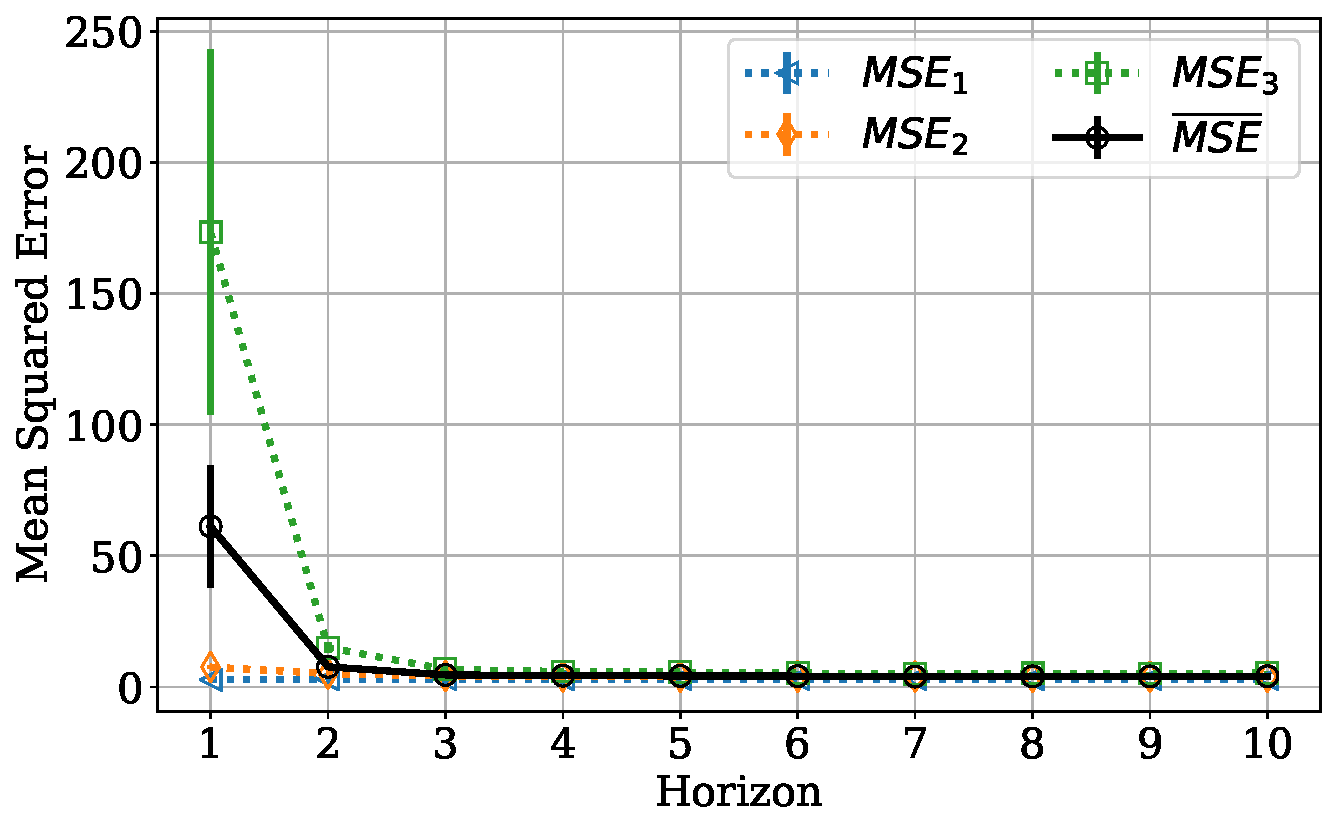
\includegraphics[width=\textwidth]{FHS2_MSE_against_H_separate}
    \caption{Scenario 2 with FHS}
  \end{subfigure}
  \hfill
  \begin{subfigure}[b]{0.49\textwidth}
    \centering
    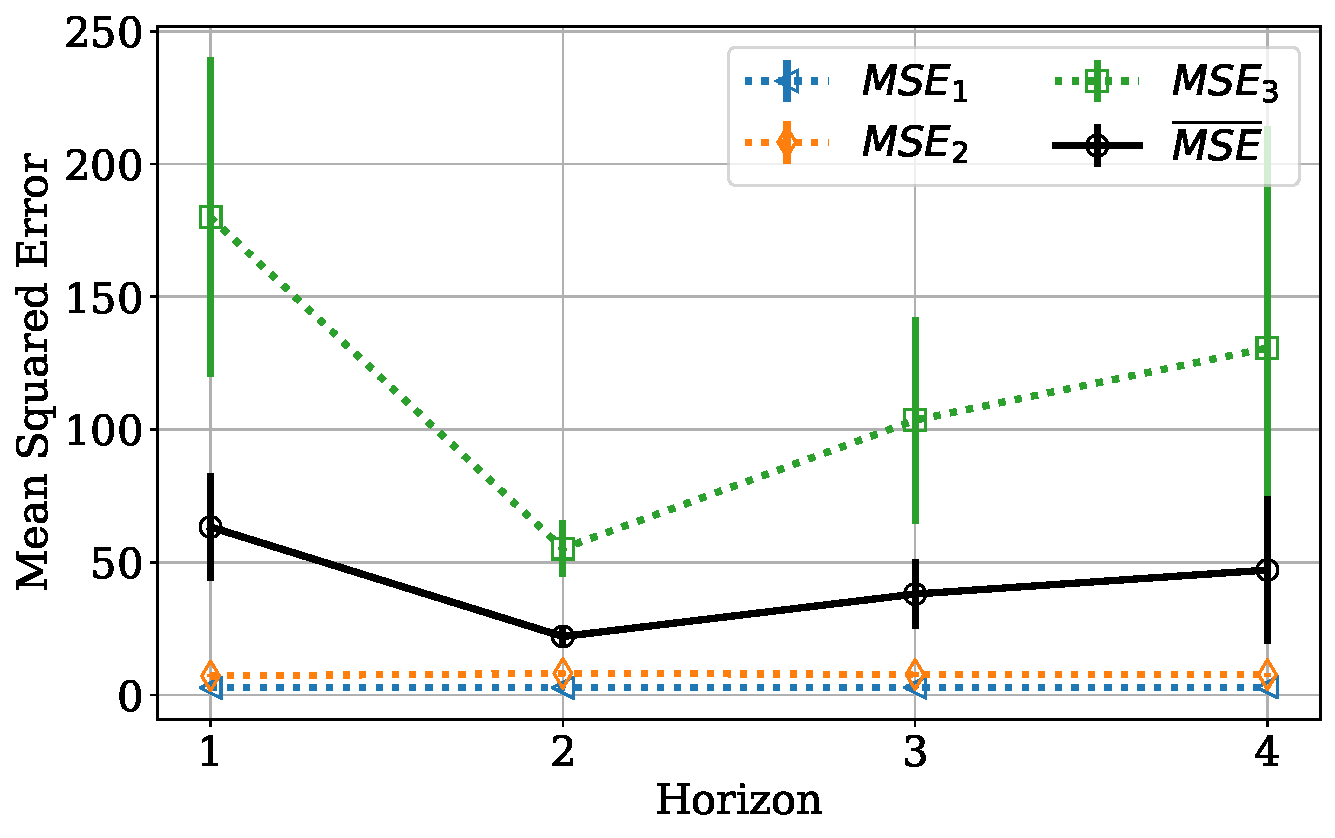
\includegraphics[width=\textwidth]{GES2_MSE_against_H_separate}
    \caption{Scenario 2 with GES}
  \end{subfigure}
  \begin{subfigure}[b]{0.49\textwidth}
    \centering
    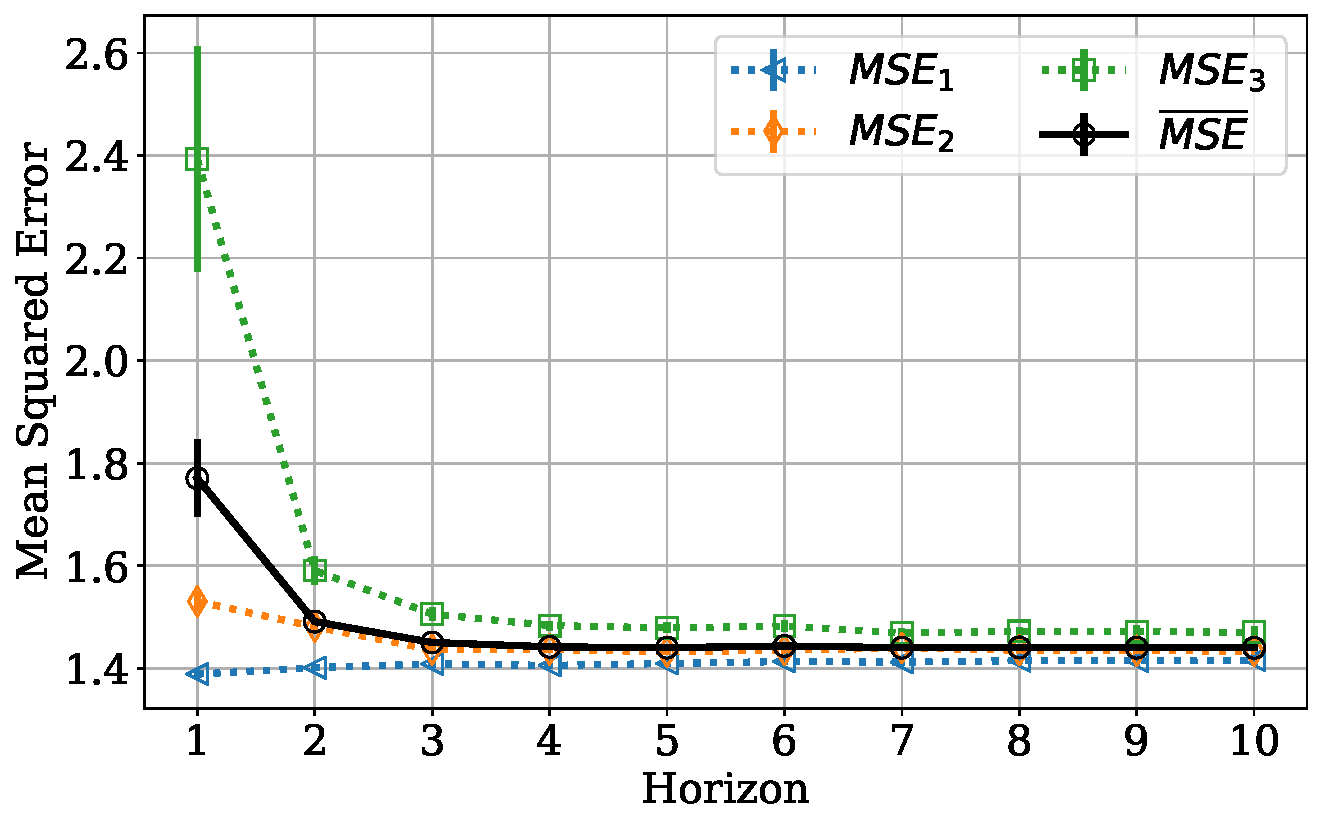
\includegraphics[width=\textwidth]{FHS3_MSE_against_H_separate}
    \caption{Scenario 3 with FHS}
  \end{subfigure}
  \hfill
  \begin{subfigure}[b]{0.49\textwidth}
    \centering
    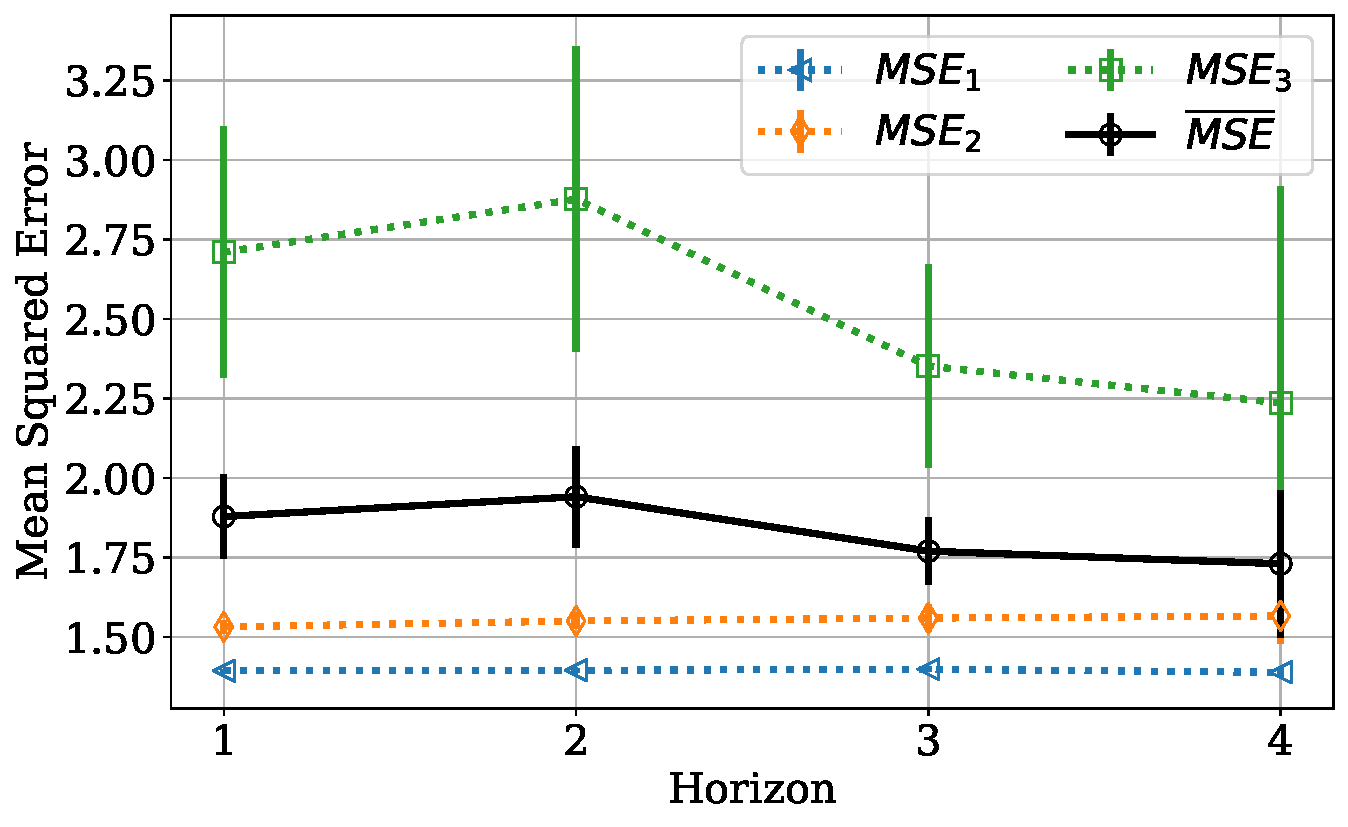
\includegraphics[width=\textwidth]{GES3_MSE_against_H_separate}
    \caption{Scenario 3 with GES}
  \end{subfigure}
  \caption{Scenario 2 \& 3: Average MSE vs. finite horizon $H$}
  \label{fig:MSEavg2}
\end{figure}

\subsection{Discussion}

It is evident that performance achieved by the proposed schedulers are
influenced by the length of burst errors. While FHS is relatively robust to
varying bursty channels, GES tends to show instable behavior. However, we can
observe the general trend that as the scheduler looks further in the future with
increasing $H$, it becomes more aware of potential high costs and adjusts
network share to prevent these.

One of the key design parameters for the proposed scheduling algorithm is the
selection of $H$. Fig.~\ref{fig:networkshare} visualizes the effect of selected
$H$ on the scheduling policy obtained from our proposed  FH scheduling scheme.
For any given finite horizon $H$ and number of control loops $N$, the size of
the underlying tree structure grows exponentially with $N\cdot H$. On the other
hand, a larger $H$ makes the scheduler more farsighted which may lead to an
improvement in performance. However, Fig.~\ref{fig:MSEavg} shows that the
expected performance gain it brings in terms of cost diminishes after a certain
$H$ value. Consequently, a finite $H$ can be chosen without losing any notable
performance gain. \\
o get an idea on how scheduler complexity increases with $H$,
Tab.~\ref{tab:complexity} compares the average number of nodes in the root tree
during simulations (GES) to its base scheduler (FHS) and the worst-case (WC)
with sampling period $D_i=1$. We observe that being fully GE-aware incurs
substantial complexity, reflected in the average node count for WC and GES. We
further notice the impact of constraining the action set as in
Eq.~\eqref{eq:admissibleactions} on the tree size. In our implementation, the
search space is reduced up to 46\% on average compared to the worst-case
scenario.

\begin{table}[htb]
  \begin{center}
  \begin{tabular}{|l|c|c|c|c|}
  \hline
  $H$ & 1 & 2 & 3 & 4 \\ 
  \hline \hline
  \textbf{GES} & 30.9 & $8.7\cdot10^2$ & $2.3\cdot10^4$ & $5.9\cdot10^5$ \\
  \textbf{FHS} & 4.6 & $17.6$ & $58.3$ & $1.9\cdot10^2$ \\
  \textbf{WC} & 33.0 & $1.1\cdot10^3$ & $3.4\cdot10^4$ & $1.1\cdot10^6$ \\
  \hline
  \end{tabular}
  \caption{Average node count of FHS and GES tree structures}
  \label{tab:complexity}
  \end{center}
\end{table}

Nevertheless, finding the optimal scheduling policy by considering every
possible network outcome is not scalable, especially for NCS scenarios with
Gilbert-Elliot channels. During evaluation we stopped GES simulations at $H=4$
as runtime were not feasible for subsequent horizons. To tackle scalability for
the proposed approach, a trade-off has to be found between optimality by
increasing H and complexity by decreasing H. In particular, the tree size has to
be reduced without neglecting possible GE channel transitions. Inspired by how
reinforcement learning copes with the \textit{exploration-exploitation dilemma},
a compromise may be found with the following idea: The complete tree structure
is built in a FHS manner in order to constrain complexity. However, we are aware
of the GE channel by augmenting the branches at certain tree levels with
transition probabilities according to GES. One could uniformly decide at each
level if a channel transition should be considered, which makes such a scheduler
``explore'' for potential performance gains instead of exploiting the
information it already has about the current channel state.

\chapter{Effect of Operating Systems on Results}

%  Conclusions (Zusammenfassung):
\chapter{Conclusion}

The thesis is concluded here. The considered problem is repeated. The
contribution of this work is highlighted and the results are recapitulated.
Remaining questions are stated and ideas for future work are expressed. 


\listoffigures
\listoftables

% Abbreviations (Abkürzungsverzeichnis):
\chapter*{Notation and Abbreviations}
% This chapter contains tables where all abbreviations and other notations like mathematical
% placeholders used in the thesis are listed.

\begin{tabular}{p{2cm} l} 
$\boldsymbol{v}^T$ & Transpose of vector $\boldsymbol{v}$\\
$\boldsymbol{M}^T$ & Transpose of matrix $\boldsymbol{M}$\\
$\tr(.)$ & Trace operator i.e. sum of all diagonal elements of a matrix\\
$\E[\mathit{X}]$ & Expected value of a random variable $\mathit{X}$\\
$\|\boldsymbol{v}\|$ & Euclidean norm of a vector $\boldsymbol{v}$ with $\|\boldsymbol{v}\|=\sqrt{\boldsymbol{v} ^T\boldsymbol{v}}$\\
$\mathcal{N}(\mu,\sigma^2)$ & Normal distribution with mean $\mu$ and standard deviation $\sigma$\\
$\mathcal{U}(a,b)$ & Uniform distribution with minimum and maximum values $a$ and $b$\\
$\Pr\left[A \mid B \right]$ & Occurrence probability of an event $A$ given $B$\\
$\mathbb{Z}^+$ & Set of positive integer numbers\\
$\mathbb{N}$ & Set of natural numbers\\
\end{tabular}
\vspace{1cm}

\hrule
\vspace{1cm}
  
\begin{tabular}{>{\bfseries}p{2cm} l}
AoI & Age-of-Information\\
BER & Bit Error Rate\\
DP & Dynamic Programming\\
FHS & Finite Horizon Scheduler\\
GE & Gilbert-Elliot\\
GES & Gilbert-Elliot Channel-aware Scheduler\\
i.i.d & independent and identically distributed\\
LTI & Linear Time-Invariant\\
MTC & Machine Type Communication\\
M2M & Machine-to-Machine\\
MSE & Mean Squared Error\\
NCS & Networked Control Systems\\
OS & Operating System\\
QoC & Quality of Control\\
VoI & Value-of-Information\\
w.r.t & with regards to\\
\end{tabular}


% References (Literaturverzeichnis):
% a) Style (with numbers: use unsrt):
\bibliographystyle{alpha}
% b) The File:
\bibliography{other/Bibliography}

% Appendix (Anhänge), could have multiple chapter-files:
% \appendix
% \chapter{}
The appendix may contain some listings of source code that has been used for simulations, extensive proofs or any other things that are strongly related to the thesis but not of immediate interest to the reader. 

%%%%%%%%%%%%%%%%%%%%%%%%%%%%%%%%%%%%%%%%%%%%%%%%%%%%%%%%%%%%


%%%%%%%%%%%%%%%%%%%%%%%%%%%%%%%%%%%%%%%%%%%%%%%%%%%%%%%%%%%%


%%%%%%%%%%%%%%%%%%%%%%%%%%%%%%%%%%%%%%%%%%%%%%%%%%%%%%%%%%%%
\end{document}
